\documentclass[twoside]{book}

% Packages required by doxygen
\usepackage{fixltx2e}
\usepackage{calc}
\usepackage{doxygen}
\usepackage[export]{adjustbox} % also loads graphicx
\usepackage{graphicx}
\usepackage[utf8]{inputenc}
\usepackage{makeidx}
\usepackage{multicol}
\usepackage{multirow}
\PassOptionsToPackage{warn}{textcomp}
\usepackage{textcomp}
\usepackage[nointegrals]{wasysym}
\usepackage[table]{xcolor}

% Font selection
\usepackage[T1]{fontenc}
\usepackage[scaled=.90]{helvet}
\usepackage{courier}
\usepackage{amssymb}
\usepackage{sectsty}
\renewcommand{\familydefault}{\sfdefault}
\allsectionsfont{%
  \fontseries{bc}\selectfont%
  \color{darkgray}%
}
\renewcommand{\DoxyLabelFont}{%
  \fontseries{bc}\selectfont%
  \color{darkgray}%
}
\newcommand{\+}{\discretionary{\mbox{\scriptsize$\hookleftarrow$}}{}{}}

% Page & text layout
\usepackage{geometry}
\geometry{%
  a4paper,%
  top=2.5cm,%
  bottom=2.5cm,%
  left=2.5cm,%
  right=2.5cm%
}
\tolerance=750
\hfuzz=15pt
\hbadness=750
\setlength{\emergencystretch}{15pt}
\setlength{\parindent}{0cm}
\setlength{\parskip}{3ex plus 2ex minus 2ex}
\makeatletter
\renewcommand{\paragraph}{%
  \@startsection{paragraph}{4}{0ex}{-1.0ex}{1.0ex}{%
    \normalfont\normalsize\bfseries\SS@parafont%
  }%
}
\renewcommand{\subparagraph}{%
  \@startsection{subparagraph}{5}{0ex}{-1.0ex}{1.0ex}{%
    \normalfont\normalsize\bfseries\SS@subparafont%
  }%
}
\makeatother

% Headers & footers
\usepackage{fancyhdr}
\pagestyle{fancyplain}
\fancyhead[LE]{\fancyplain{}{\bfseries\thepage}}
\fancyhead[CE]{\fancyplain{}{}}
\fancyhead[RE]{\fancyplain{}{\bfseries\leftmark}}
\fancyhead[LO]{\fancyplain{}{\bfseries\rightmark}}
\fancyhead[CO]{\fancyplain{}{}}
\fancyhead[RO]{\fancyplain{}{\bfseries\thepage}}
\fancyfoot[LE]{\fancyplain{}{}}
\fancyfoot[CE]{\fancyplain{}{}}
\fancyfoot[RE]{\fancyplain{}{\bfseries\scriptsize Generated by Doxygen }}
\fancyfoot[LO]{\fancyplain{}{\bfseries\scriptsize Generated by Doxygen }}
\fancyfoot[CO]{\fancyplain{}{}}
\fancyfoot[RO]{\fancyplain{}{}}
\renewcommand{\footrulewidth}{0.4pt}
\renewcommand{\chaptermark}[1]{%
  \markboth{#1}{}%
}
\renewcommand{\sectionmark}[1]{%
  \markright{\thesection\ #1}%
}

% Indices & bibliography
\usepackage{natbib}
\usepackage[titles]{tocloft}
\setcounter{tocdepth}{3}
\setcounter{secnumdepth}{5}
\makeindex

% Hyperlinks (required, but should be loaded last)
\usepackage{ifpdf}
\ifpdf
  \usepackage[pdftex,pagebackref=true]{hyperref}
\else
  \usepackage[ps2pdf,pagebackref=true]{hyperref}
\fi
\hypersetup{%
  colorlinks=true,%
  linkcolor=blue,%
  citecolor=blue,%
  unicode%
}

% Custom commands
\newcommand{\clearemptydoublepage}{%
  \newpage{\pagestyle{empty}\cleardoublepage}%
}

\usepackage{caption}
\captionsetup{labelsep=space,justification=centering,font={bf},singlelinecheck=off,skip=4pt,position=top}

%===== C O N T E N T S =====

\begin{document}

% Titlepage & ToC
\hypersetup{pageanchor=false,
             bookmarksnumbered=true,
             pdfencoding=unicode
            }
\pagenumbering{alph}
\begin{titlepage}
\vspace*{7cm}
\begin{center}%
{\Large Taxis }\\
\vspace*{1cm}
{\large Generated by Doxygen 1.8.12}\\
\end{center}
\end{titlepage}
\clearemptydoublepage
\pagenumbering{roman}
\tableofcontents
\clearemptydoublepage
\pagenumbering{arabic}
\hypersetup{pageanchor=true}

%--- Begin generated contents ---
\chapter{Hierarchical Index}
\section{Class Hierarchy}
This inheritance list is sorted roughly, but not completely, alphabetically\+:\begin{DoxyCompactList}
\item \contentsline{section}{Binary\+Node$<$ Comparable $>$}{\pageref{class_binary_node}}{}
\item \contentsline{section}{Binary\+Node$<$ Servico\+Pointer $\ast$$>$}{\pageref{class_binary_node}}{}
\item \contentsline{section}{B\+ST$<$ Comparable $>$}{\pageref{class_b_s_t}}{}
\item \contentsline{section}{B\+ST$<$ Servico\+Pointer $\ast$$>$}{\pageref{class_b_s_t}}{}
\item \contentsline{section}{B\+S\+T\+Itr\+In$<$ Comparable $>$}{\pageref{class_b_s_t_itr_in}}{}
\item \contentsline{section}{B\+S\+T\+Itr\+Level$<$ Comparable $>$}{\pageref{class_b_s_t_itr_level}}{}
\item \contentsline{section}{B\+S\+T\+Itr\+Post$<$ Comparable $>$}{\pageref{class_b_s_t_itr_post}}{}
\item \contentsline{section}{B\+S\+T\+Itr\+Pre$<$ Comparable $>$}{\pageref{class_b_s_t_itr_pre}}{}
\item \contentsline{section}{Cliente}{\pageref{class_cliente}}{}
\begin{DoxyCompactList}
\item \contentsline{section}{Registado}{\pageref{class_registado}}{}
\begin{DoxyCompactList}
\item \contentsline{section}{Empresarial}{\pageref{class_empresarial}}{}
\item \contentsline{section}{Particular}{\pageref{class_particular}}{}
\end{DoxyCompactList}
\end{DoxyCompactList}
\item \contentsline{section}{Cliente\+Inexistente}{\pageref{class_cliente_inexistente}}{}
\item \contentsline{section}{Cliente\+Repetido}{\pageref{class_cliente_repetido}}{}
\item \contentsline{section}{data\+\_\+struct}{\pageref{structdata__struct}}{}
\item \contentsline{section}{Empresa}{\pageref{class_empresa}}{}
\item \contentsline{section}{h\+Registado\+Pointer}{\pageref{structh_registado_pointer}}{}
\item \contentsline{section}{Interface}{\pageref{class_interface}}{}
\item \contentsline{section}{Registado\+Pointer}{\pageref{class_registado_pointer}}{}
\item \contentsline{section}{Servico}{\pageref{class_servico}}{}
\item \contentsline{section}{Servico\+Pointer}{\pageref{class_servico_pointer}}{}
\item \contentsline{section}{tempo}{\pageref{structtempo}}{}
\end{DoxyCompactList}

\chapter{Class Index}
\section{Class List}
Here are the classes, structs, unions and interfaces with brief descriptions\+:\begin{DoxyCompactList}
\item\contentsline{section}{\hyperlink{class_cliente}{Cliente} }{\pageref{class_cliente}}{}
\item\contentsline{section}{\hyperlink{class_cliente_inexistente}{Cliente\+Inexistente} }{\pageref{class_cliente_inexistente}}{}
\item\contentsline{section}{\hyperlink{class_cliente_repetido}{Cliente\+Repetido} }{\pageref{class_cliente_repetido}}{}
\item\contentsline{section}{\hyperlink{structdata__struct}{data\+\_\+struct} }{\pageref{structdata__struct}}{}
\item\contentsline{section}{\hyperlink{class_empresa}{Empresa} }{\pageref{class_empresa}}{}
\item\contentsline{section}{\hyperlink{class_empresarial}{Empresarial} }{\pageref{class_empresarial}}{}
\item\contentsline{section}{\hyperlink{class_interface}{Interface} }{\pageref{class_interface}}{}
\item\contentsline{section}{\hyperlink{class_particular}{Particular} }{\pageref{class_particular}}{}
\item\contentsline{section}{\hyperlink{class_registado}{Registado} }{\pageref{class_registado}}{}
\item\contentsline{section}{\hyperlink{class_servico}{Servico} }{\pageref{class_servico}}{}
\item\contentsline{section}{\hyperlink{structtempo}{tempo} }{\pageref{structtempo}}{}
\end{DoxyCompactList}

\chapter{Class Documentation}
\hypertarget{class_cliente}{}\section{Cliente Class Reference}
\label{class_cliente}\index{Cliente@{Cliente}}
Inheritance diagram for Cliente\+:\begin{figure}[H]
\begin{center}
\leavevmode
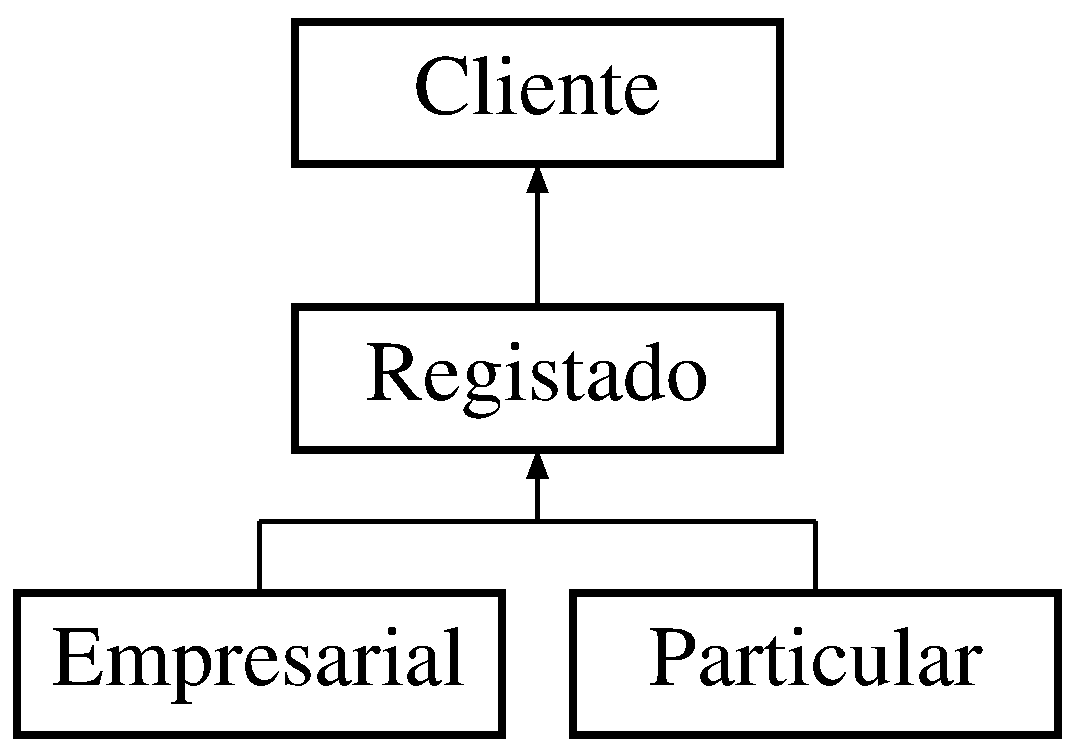
\includegraphics[height=3.000000cm]{class_cliente}
\end{center}
\end{figure}
\subsection*{Public Member Functions}
\begin{DoxyCompactItemize}
\item 
\hyperlink{class_cliente_a5957c05b3d3594a7cbd8c088486d14ae}{Cliente} (const std\+::string nome, const std\+::string morada, const unsigned int N\+IF)
\item 
\hyperlink{class_cliente_a030699a841488d4b3dfbedf75834e002}{Cliente} (const std\+::string nome, const std\+::string morada)
\item 
\hyperlink{class_cliente_a17e05e34ce319b738fb68c53e4ded2c3}{Cliente} (std\+::string nome)
\item 
\hypertarget{class_cliente_a7972b72a8288e5dee92b30579017c549}{}\label{class_cliente_a7972b72a8288e5dee92b30579017c549} 
bool {\bfseries operator==} (const \hyperlink{class_cliente}{Cliente} \&cli) const
\item 
\hypertarget{class_cliente_aa1c8490c22c31b6c7ccdb794cadc866d}{}\label{class_cliente_aa1c8490c22c31b6c7ccdb794cadc866d} 
bool {\bfseries operator$<$} (const \hyperlink{class_cliente}{Cliente} \&cli) const
\item 
void \hyperlink{class_cliente_a3aa84b64135b106669724fc08b7cc91f}{operator=} (const \hyperlink{class_cliente}{Cliente} \&cli)
\item 
\hypertarget{class_cliente_abfd45b8b07a8549fe4761d00c76a43c3}{}\label{class_cliente_abfd45b8b07a8549fe4761d00c76a43c3} 
std\+::string {\bfseries get\+Nome} () const
\item 
\hypertarget{class_cliente_af73bfd0b9fc0f7facf4f6d9acbe757b1}{}\label{class_cliente_af73bfd0b9fc0f7facf4f6d9acbe757b1} 
std\+::string {\bfseries get\+Morada} () const
\item 
\hypertarget{class_cliente_a8dedf04f5520b5849ecd70a1c4d07a86}{}\label{class_cliente_a8dedf04f5520b5849ecd70a1c4d07a86} 
unsigned int {\bfseries get\+N\+IF} () const
\item 
virtual std\+::string \hyperlink{class_cliente_a932ef71b2792dc5df153f82d3e81a6f3}{get\+Informacao} () const
\item 
\hypertarget{class_cliente_a6f69591975dd6db60d61da4744a61d95}{}\label{class_cliente_a6f69591975dd6db60d61da4744a61d95} 
void {\bfseries set\+Nome} (std\+::string nome)
\item 
\hypertarget{class_cliente_ac153d8134504564bb599d47611cd7726}{}\label{class_cliente_ac153d8134504564bb599d47611cd7726} 
void {\bfseries set\+Morada} (std\+::string morada)
\item 
\hypertarget{class_cliente_a203e0f379622d73f1f58f2d650233a8d}{}\label{class_cliente_a203e0f379622d73f1f58f2d650233a8d} 
void {\bfseries set\+N\+IF} (unsigned int N\+IF)
\item 
virtual bool \hyperlink{class_cliente_a68646846a80de5cdcb61b1f8a13e4fb8}{pagamento\+Numerario} (\hyperlink{class_servico}{Servico} \&serv)
\item 
virtual bool \hyperlink{class_cliente_a6e230e5e512bebe07bfa1ad6750b8cee}{pagamento\+Multibanco} (\hyperlink{class_servico}{Servico} \&serv)
\end{DoxyCompactItemize}
\subsection*{Protected Attributes}
\begin{DoxyCompactItemize}
\item 
\hypertarget{class_cliente_aaa79b0a26f7d5d007fe4ae9696564ca5}{}\label{class_cliente_aaa79b0a26f7d5d007fe4ae9696564ca5} 
std\+::string {\bfseries nome}
\item 
\hypertarget{class_cliente_a24ba6895be9bdf5112e9e67a34d13704}{}\label{class_cliente_a24ba6895be9bdf5112e9e67a34d13704} 
std\+::string {\bfseries morada}
\item 
\hypertarget{class_cliente_a7a012a7819f17eb18a9580fe32723aeb}{}\label{class_cliente_a7a012a7819f17eb18a9580fe32723aeb} 
unsigned int {\bfseries N\+IF}
\end{DoxyCompactItemize}


\subsection{Constructor \& Destructor Documentation}
\hypertarget{class_cliente_a5957c05b3d3594a7cbd8c088486d14ae}{}\label{class_cliente_a5957c05b3d3594a7cbd8c088486d14ae} 
\index{Cliente@{Cliente}!Cliente@{Cliente}}
\index{Cliente@{Cliente}!Cliente@{Cliente}}
\subsubsection{\texorpdfstring{Cliente()}{Cliente()}\hspace{0.1cm}{\footnotesize\ttfamily [1/3]}}
{\footnotesize\ttfamily Cliente\+::\+Cliente (\begin{DoxyParamCaption}\item[{const std\+::string}]{nome,  }\item[{const std\+::string}]{morada,  }\item[{const unsigned int}]{N\+IF }\end{DoxyParamCaption})}

Constructor de clienete 
\begin{DoxyParams}{Parameters}
{\em nome,morada,N\+IF} & \\
\hline
\end{DoxyParams}
\hypertarget{class_cliente_a030699a841488d4b3dfbedf75834e002}{}\label{class_cliente_a030699a841488d4b3dfbedf75834e002} 
\index{Cliente@{Cliente}!Cliente@{Cliente}}
\index{Cliente@{Cliente}!Cliente@{Cliente}}
\subsubsection{\texorpdfstring{Cliente()}{Cliente()}\hspace{0.1cm}{\footnotesize\ttfamily [2/3]}}
{\footnotesize\ttfamily Cliente\+::\+Cliente (\begin{DoxyParamCaption}\item[{const std\+::string}]{nome,  }\item[{const std\+::string}]{morada }\end{DoxyParamCaption})}

Constructor de clienete 
\begin{DoxyParams}{Parameters}
{\em nome,morada} & pode ser usado para clientes nao registados \\
\hline
\end{DoxyParams}
\hypertarget{class_cliente_a17e05e34ce319b738fb68c53e4ded2c3}{}\label{class_cliente_a17e05e34ce319b738fb68c53e4ded2c3} 
\index{Cliente@{Cliente}!Cliente@{Cliente}}
\index{Cliente@{Cliente}!Cliente@{Cliente}}
\subsubsection{\texorpdfstring{Cliente()}{Cliente()}\hspace{0.1cm}{\footnotesize\ttfamily [3/3]}}
{\footnotesize\ttfamily Cliente\+::\+Cliente (\begin{DoxyParamCaption}\item[{std\+::string}]{nome }\end{DoxyParamCaption})}

Constructor de clienete 
\begin{DoxyParams}{Parameters}
{\em nome} & pode ser usado para clientes nao registados \\
\hline
\end{DoxyParams}


\subsection{Member Function Documentation}
\hypertarget{class_cliente_a932ef71b2792dc5df153f82d3e81a6f3}{}\label{class_cliente_a932ef71b2792dc5df153f82d3e81a6f3} 
\index{Cliente@{Cliente}!get\+Informacao@{get\+Informacao}}
\index{get\+Informacao@{get\+Informacao}!Cliente@{Cliente}}
\subsubsection{\texorpdfstring{get\+Informacao()}{getInformacao()}}
{\footnotesize\ttfamily std\+::string Cliente\+::get\+Informacao (\begin{DoxyParamCaption}{ }\end{DoxyParamCaption}) const\hspace{0.3cm}{\ttfamily [virtual]}}

Informacao relativa a um cliente

\begin{DoxyReturn}{Returns}
uma string com a morada, nome e N\+IF de um cliente, ja formatadoa 
\end{DoxyReturn}


Reimplemented in \hyperlink{class_particular_acde85dcb3d26ca3afe131fb4c35763c8}{Particular}, \hyperlink{class_empresarial_a28090b6b3db16b6b7ba03d6308c2c309}{Empresarial}, and \hyperlink{class_registado_a7017f0d74afd44459c3d6affcb303d52}{Registado}.

\hypertarget{class_cliente_a3aa84b64135b106669724fc08b7cc91f}{}\label{class_cliente_a3aa84b64135b106669724fc08b7cc91f} 
\index{Cliente@{Cliente}!operator=@{operator=}}
\index{operator=@{operator=}!Cliente@{Cliente}}
\subsubsection{\texorpdfstring{operator=()}{operator=()}}
{\footnotesize\ttfamily void Cliente\+::operator= (\begin{DoxyParamCaption}\item[{const \hyperlink{class_cliente}{Cliente} \&}]{cli }\end{DoxyParamCaption})}

Operator =


\begin{DoxyParams}{Parameters}
{\em cli} & iguala o nome e a morada de um cliente ao nome e morada de outro cliente \\
\hline
\end{DoxyParams}
\hypertarget{class_cliente_a6e230e5e512bebe07bfa1ad6750b8cee}{}\label{class_cliente_a6e230e5e512bebe07bfa1ad6750b8cee} 
\index{Cliente@{Cliente}!pagamento\+Multibanco@{pagamento\+Multibanco}}
\index{pagamento\+Multibanco@{pagamento\+Multibanco}!Cliente@{Cliente}}
\subsubsection{\texorpdfstring{pagamento\+Multibanco()}{pagamentoMultibanco()}}
{\footnotesize\ttfamily bool Cliente\+::pagamento\+Multibanco (\begin{DoxyParamCaption}\item[{\hyperlink{class_servico}{Servico} \&}]{serv }\end{DoxyParamCaption})\hspace{0.3cm}{\ttfamily [virtual]}}

Constructor de clienete 
\begin{DoxyParams}{Parameters}
{\em nome,morada,N\+IF} & \\
\hline
\end{DoxyParams}


Reimplemented in \hyperlink{class_registado_a36be4ccf8e4b1bc26be7c1c2d4612229}{Registado}.

\hypertarget{class_cliente_a68646846a80de5cdcb61b1f8a13e4fb8}{}\label{class_cliente_a68646846a80de5cdcb61b1f8a13e4fb8} 
\index{Cliente@{Cliente}!pagamento\+Numerario@{pagamento\+Numerario}}
\index{pagamento\+Numerario@{pagamento\+Numerario}!Cliente@{Cliente}}
\subsubsection{\texorpdfstring{pagamento\+Numerario()}{pagamentoNumerario()}}
{\footnotesize\ttfamily bool Cliente\+::pagamento\+Numerario (\begin{DoxyParamCaption}\item[{\hyperlink{class_servico}{Servico} \&}]{serv }\end{DoxyParamCaption})\hspace{0.3cm}{\ttfamily [virtual]}}

Pagamento de um servico em numerario


\begin{DoxyParams}{Parameters}
{\em serv} & efectua o pagamento do servico lancado como argumento pelo metodo de numerario atribui ao N\+IF do servico o N\+IF do cliente que o pagou, para ser guardado na empresa \\
\hline
\end{DoxyParams}


Reimplemented in \hyperlink{class_registado_af3c8f63f7df1cdfd27e44126f78b71d8}{Registado}.



The documentation for this class was generated from the following files\+:\begin{DoxyCompactItemize}
\item 
C\+:/\+Users/\+User\+Candido/\+Desktop/\+Eclipse A\+E\+D\+A/\+C\+A\+L/\+Taxis 2/src/Cliente.\+h\item 
C\+:/\+Users/\+User\+Candido/\+Desktop/\+Eclipse A\+E\+D\+A/\+C\+A\+L/\+Taxis 2/src/Cliente.\+cpp\end{DoxyCompactItemize}

\hypertarget{class_cliente_inexistente}{}\section{Cliente\+Inexistente Class Reference}
\label{class_cliente_inexistente}\index{Cliente\+Inexistente@{Cliente\+Inexistente}}
\subsection*{Public Member Functions}
\begin{DoxyCompactItemize}
\item 
\mbox{\Hypertarget{class_cliente_inexistente_af0451741cd6c658bfe981c2589ca6285}\label{class_cliente_inexistente_af0451741cd6c658bfe981c2589ca6285}} 
{\bfseries Cliente\+Inexistente} (std\+::string nome, std\+::string morada)
\item 
\mbox{\Hypertarget{class_cliente_inexistente_a0792c70fde5b7f2e29ccad035acaa7b8}\label{class_cliente_inexistente_a0792c70fde5b7f2e29ccad035acaa7b8}} 
{\bfseries Cliente\+Inexistente} (std\+::string nome, std\+::string morada, unsigned int N\+IF)
\item 
\mbox{\Hypertarget{class_cliente_inexistente_a41daf5a590224c14a40329686ff2e0e6}\label{class_cliente_inexistente_a41daf5a590224c14a40329686ff2e0e6}} 
void {\bfseries print\+Info} ()
\end{DoxyCompactItemize}
\subsection*{Private Attributes}
\begin{DoxyCompactItemize}
\item 
\mbox{\Hypertarget{class_cliente_inexistente_acb18f88084236fd6ecfc9af59605c4d8}\label{class_cliente_inexistente_acb18f88084236fd6ecfc9af59605c4d8}} 
std\+::string {\bfseries nome}
\item 
\mbox{\Hypertarget{class_cliente_inexistente_a562fb3314372bea473711dc6b50641d8}\label{class_cliente_inexistente_a562fb3314372bea473711dc6b50641d8}} 
std\+::string {\bfseries morada}
\item 
\mbox{\Hypertarget{class_cliente_inexistente_ad64664c5a6ac9cf9f4b5d3991ddbb7fd}\label{class_cliente_inexistente_ad64664c5a6ac9cf9f4b5d3991ddbb7fd}} 
unsigned int {\bfseries N\+IF}
\end{DoxyCompactItemize}


The documentation for this class was generated from the following file\+:\begin{DoxyCompactItemize}
\item 
C\+:/\+Users/user/\+Desktop/\+Taxis src/src/Empresa.\+h\end{DoxyCompactItemize}

\hypertarget{class_cliente_repetido}{}\section{Cliente\+Repetido Class Reference}
\label{class_cliente_repetido}\index{Cliente\+Repetido@{Cliente\+Repetido}}
\subsection*{Public Member Functions}
\begin{DoxyCompactItemize}
\item 
\hypertarget{class_cliente_repetido_a9cea00e5f8ccbdc17b1255c18b0db76a}{}\label{class_cliente_repetido_a9cea00e5f8ccbdc17b1255c18b0db76a} 
{\bfseries Cliente\+Repetido} (std\+::string nome, std\+::string morada)
\item 
\hypertarget{class_cliente_repetido_aef162764c8915bc8b828819810dfb244}{}\label{class_cliente_repetido_aef162764c8915bc8b828819810dfb244} 
{\bfseries Cliente\+Repetido} (std\+::string nome, std\+::string morada, unsigned int N\+IF)
\item 
\hypertarget{class_cliente_repetido_aaf0c377313c9c28280c9f31c2e390f9c}{}\label{class_cliente_repetido_aaf0c377313c9c28280c9f31c2e390f9c} 
void {\bfseries print\+Info} ()
\end{DoxyCompactItemize}
\subsection*{Private Attributes}
\begin{DoxyCompactItemize}
\item 
\hypertarget{class_cliente_repetido_a2456d62012c9fb5059eb3e55563ba73d}{}\label{class_cliente_repetido_a2456d62012c9fb5059eb3e55563ba73d} 
std\+::string {\bfseries nome}
\item 
\hypertarget{class_cliente_repetido_af103299aa577b7be308b4acfa394805f}{}\label{class_cliente_repetido_af103299aa577b7be308b4acfa394805f} 
std\+::string {\bfseries morada}
\item 
\hypertarget{class_cliente_repetido_a3741557d88f69acdec3ef7c7a1f47fe6}{}\label{class_cliente_repetido_a3741557d88f69acdec3ef7c7a1f47fe6} 
unsigned int {\bfseries N\+IF}
\end{DoxyCompactItemize}


The documentation for this class was generated from the following file\+:\begin{DoxyCompactItemize}
\item 
C\+:/\+Users/\+User\+Candido/\+Desktop/\+Eclipse A\+E\+D\+A/\+C\+A\+L/\+Taxis 2/src/Empresa.\+h\end{DoxyCompactItemize}

\hypertarget{structdata__struct}{}\section{data\+\_\+struct Struct Reference}
\label{structdata__struct}\index{data\+\_\+struct@{data\+\_\+struct}}
\subsection*{Public Attributes}
\begin{DoxyCompactItemize}
\item 
\hypertarget{structdata__struct_a17a70fb8ce7ea58aff3b0ba60b7f5e5b}{}\label{structdata__struct_a17a70fb8ce7ea58aff3b0ba60b7f5e5b} 
unsigned int {\bfseries dia}
\item 
\hypertarget{structdata__struct_a07c99afd664b3c1d36462e87201f2a89}{}\label{structdata__struct_a07c99afd664b3c1d36462e87201f2a89} 
unsigned int {\bfseries mes}
\item 
\hypertarget{structdata__struct_a1d3ed5c9543d622a7ed8785f8007f8f9}{}\label{structdata__struct_a1d3ed5c9543d622a7ed8785f8007f8f9} 
unsigned int {\bfseries ano}
\end{DoxyCompactItemize}


The documentation for this struct was generated from the following file\+:\begin{DoxyCompactItemize}
\item 
C\+:/\+Users/\+User\+Candido/\+Desktop/\+Eclipse A\+E\+D\+A/\+C\+A\+L/\+Taxis 2/src/Utilidades.\+h\end{DoxyCompactItemize}

\hypertarget{class_empresa}{}\section{Empresa Class Reference}
\label{class_empresa}\index{Empresa@{Empresa}}
\subsection*{Public Member Functions}
\begin{DoxyCompactItemize}
\item 
\mbox{\Hypertarget{class_empresa_a246d93027070baa8adfd65d16aa4199d}\label{class_empresa_a246d93027070baa8adfd65d16aa4199d}} 
{\bfseries Empresa} (std\+::string nome)
\item 
\mbox{\Hypertarget{class_empresa_a84deac5a4a2151c58759f89167a45124}\label{class_empresa_a84deac5a4a2151c58759f89167a45124}} 
{\bfseries Empresa} (std\+::string nome, std\+::string morada)
\item 
\mbox{\Hypertarget{class_empresa_a7c9543608b1bc26bab8f4ad8c6d28128}\label{class_empresa_a7c9543608b1bc26bab8f4ad8c6d28128}} 
void {\bfseries set\+Nome} (std\+::string nome)
\item 
\mbox{\Hypertarget{class_empresa_a5bd86d8ec03de652cfd11797de5bbe22}\label{class_empresa_a5bd86d8ec03de652cfd11797de5bbe22}} 
void {\bfseries set\+Morada} (std\+::string morada)
\item 
\mbox{\Hypertarget{class_empresa_ae917f6b8a8be9316e1dd553b2ccb6332}\label{class_empresa_ae917f6b8a8be9316e1dd553b2ccb6332}} 
std\+::string {\bfseries get\+Nome} () const
\item 
\mbox{\Hypertarget{class_empresa_a4ba5753ee333e062a47615b0a2c442c2}\label{class_empresa_a4ba5753ee333e062a47615b0a2c442c2}} 
std\+::string {\bfseries get\+Morada} () const
\item 
\mbox{\Hypertarget{class_empresa_a7625bb6835dec408801b92e0f6ae89bb}\label{class_empresa_a7625bb6835dec408801b92e0f6ae89bb}} 
std\+::vector$<$ \hyperlink{class_registado}{Registado} $\ast$ $>$ {\bfseries get\+Registados} () const
\item 
\mbox{\Hypertarget{class_empresa_a35b2ad7ce666b30d99edd10c691b335a}\label{class_empresa_a35b2ad7ce666b30d99edd10c691b335a}} 
\hyperlink{class_registado}{Registado} $\ast$ {\bfseries get\+Registado\+By\+N\+IF} (unsigned int N\+IF) const
\item 
\mbox{\Hypertarget{class_empresa_a6057325975eae633f66ba2504ac8dd09}\label{class_empresa_a6057325975eae633f66ba2504ac8dd09}} 
\hyperlink{class_servico}{Servico} $\ast$ {\bfseries get\+Servico\+By\+ID} (unsigned int serv\+ID) const
\item 
\mbox{\Hypertarget{class_empresa_ae9df2a1a1d8bf2ac64d08a88a13f0c5f}\label{class_empresa_ae9df2a1a1d8bf2ac64d08a88a13f0c5f}} 
bool {\bfseries adiciona\+Cliente} (\hyperlink{class_registado}{Registado} $\ast$cli)
\item 
\mbox{\Hypertarget{class_empresa_aec387d18fb6dc010738c5d878cff1645}\label{class_empresa_aec387d18fb6dc010738c5d878cff1645}} 
bool {\bfseries remove\+Cliente} (\hyperlink{class_registado}{Registado} $\ast$cli)
\item 
\mbox{\Hypertarget{class_empresa_ad92331511c58763afed45f668421454c}\label{class_empresa_ad92331511c58763afed45f668421454c}} 
bool {\bfseries remove\+Cliente} (unsigned int N\+IF)
\item 
\mbox{\Hypertarget{class_empresa_a1f97b7763f0d4977192713a6350d45c4}\label{class_empresa_a1f97b7763f0d4977192713a6350d45c4}} 
std\+::vector$<$ \hyperlink{class_servico}{Servico} $\ast$ $>$ {\bfseries get\+Historico} () const
\item 
\mbox{\Hypertarget{class_empresa_a31c9add956cf208592c82e600389ebec}\label{class_empresa_a31c9add956cf208592c82e600389ebec}} 
std\+::string {\bfseries get\+Informacao} () const
\item 
\mbox{\Hypertarget{class_empresa_a3a0b6dad40b7f05fede47be28dfc024d}\label{class_empresa_a3a0b6dad40b7f05fede47be28dfc024d}} 
std\+::string {\bfseries get\+Informacao\+Servicos} () const
\item 
\mbox{\Hypertarget{class_empresa_a670edd3a8103ef4136a5d59054018278}\label{class_empresa_a670edd3a8103ef4136a5d59054018278}} 
std\+::string {\bfseries get\+N\+I\+Fs\+Clientes} () const
\item 
\mbox{\Hypertarget{class_empresa_a601351adee76c9258438f841a41c5eaa}\label{class_empresa_a601351adee76c9258438f841a41c5eaa}} 
std\+::string {\bfseries get\+I\+Ds\+Servicos} () const
\item 
\mbox{\Hypertarget{class_empresa_af40fde81230d4c58c678c3bfb6b1b35b}\label{class_empresa_af40fde81230d4c58c678c3bfb6b1b35b}} 
std\+::string {\bfseries get\+Servicos\+By\+Cliente} (unsigned int N\+IF) const
\item 
\mbox{\Hypertarget{class_empresa_ae7e7f8be439aa63d7c6b174818260e32}\label{class_empresa_ae7e7f8be439aa63d7c6b174818260e32}} 
bool {\bfseries adiciona\+Servico\+Cliente} (\hyperlink{class_servico}{Servico} $\ast$serv, unsigned int N\+IF)
\item 
\mbox{\Hypertarget{class_empresa_a17638d7cbc03ab5f6e0a4a57bb99ca56}\label{class_empresa_a17638d7cbc03ab5f6e0a4a57bb99ca56}} 
bool {\bfseries servico\+Rapido} (\hyperlink{class_servico}{Servico} $\ast$serv, \hyperlink{class_cliente}{Cliente} $\ast$cli, std\+::string metodo\+\_\+pagamento)
\item 
\mbox{\Hypertarget{class_empresa_a1ea3f3759f3377ba18c974b21254c8e6}\label{class_empresa_a1ea3f3759f3377ba18c974b21254c8e6}} 
bool {\bfseries pagamento\+Servico\+Cliente} (unsigned int N\+IF)
\item 
\mbox{\Hypertarget{class_empresa_a27262bddd41ff48b0585e05ef600e9fe}\label{class_empresa_a27262bddd41ff48b0585e05ef600e9fe}} 
bool {\bfseries set\+Nome\+Servico} (std\+::string nome, unsigned int serv\+ID)
\item 
\hyperlink{class_b_s_t}{B\+ST}$<$ \hyperlink{class_servico_pointer}{Servico\+Pointer} $\ast$ $>$ \hyperlink{class_empresa_a1515dc722b64eab75b9d7a37ddd7863b}{get\+Arvore\+Servicos} () const
\begin{DoxyCompactList}\small\item\em retorna \hyperlink{class_b_s_t}{B\+ST} de servicos da empresa \end{DoxyCompactList}\item 
bool \hyperlink{class_empresa_a7f40b739ea88afe971c3a52d520d708a}{add\+Servico\+B\+ST} (\hyperlink{class_servico}{Servico} $\ast$serv)
\begin{DoxyCompactList}\small\item\em adiciona um servico a \hyperlink{class_b_s_t}{B\+ST} de servicos da empresa /$\ast$ \end{DoxyCompactList}\item 
void \hyperlink{class_empresa_a7e760a09feabb76e7ab0b121be61be4a}{print\+Arvore\+Servicos} () const
\begin{DoxyCompactList}\small\item\em imprime informacao sobre a \hyperlink{class_b_s_t}{B\+ST} de servicos da empresa \end{DoxyCompactList}\item 
void \hyperlink{class_empresa_a218427b819a92be11e5f1c808dcd3153}{update\+Arvore\+Servicos} ()
\begin{DoxyCompactList}\small\item\em atualiza \hyperlink{class_b_s_t}{B\+ST} de servicos da empresa \end{DoxyCompactList}\item 
tab\+H\+Cliente \hyperlink{class_empresa_aeb8ed69f2ec85275de6372e18a8945db}{get\+Tabela\+Clientes\+Inativos} () const
\begin{DoxyCompactList}\small\item\em retorna hash table de clientes inativos da empresa \end{DoxyCompactList}\item 
void \hyperlink{class_empresa_a232b5da45afd7aad19ab503210b0c922}{print\+Tabela\+Clientes\+Inativos} () const
\begin{DoxyCompactList}\small\item\em imprime informacao relativa a hash table de clientes inativos da empresa \end{DoxyCompactList}\item 
bool \hyperlink{class_empresa_a99f0d3892ad29e4c44e72f14189c4388}{update\+Tabela\+Clientes\+Inativos} ()
\begin{DoxyCompactList}\small\item\em atualiza hash table de clientes inativos da empresa \end{DoxyCompactList}\end{DoxyCompactItemize}
\subsection*{Private Attributes}
\begin{DoxyCompactItemize}
\item 
\mbox{\Hypertarget{class_empresa_affa32f93b722be794531dbfb26cb19b3}\label{class_empresa_affa32f93b722be794531dbfb26cb19b3}} 
std\+::string {\bfseries nome}
\item 
\mbox{\Hypertarget{class_empresa_a73cf106d1c427875d58d7adc0ff298e8}\label{class_empresa_a73cf106d1c427875d58d7adc0ff298e8}} 
std\+::string {\bfseries morada}
\item 
\mbox{\Hypertarget{class_empresa_aed45bb351ecd8503398d43c7da1487f8}\label{class_empresa_aed45bb351ecd8503398d43c7da1487f8}} 
std\+::vector$<$ \hyperlink{class_registado}{Registado} $\ast$ $>$ {\bfseries clientes}
\item 
\mbox{\Hypertarget{class_empresa_ae8b0f4fece7e5c01d136ab79418f728b}\label{class_empresa_ae8b0f4fece7e5c01d136ab79418f728b}} 
std\+::vector$<$ \hyperlink{class_servico}{Servico} $\ast$ $>$ {\bfseries historico}
\item 
\mbox{\Hypertarget{class_empresa_ae7a1dd04902ed33525db1c6400cade59}\label{class_empresa_ae7a1dd04902ed33525db1c6400cade59}} 
\hyperlink{class_b_s_t}{B\+ST}$<$ \hyperlink{class_servico_pointer}{Servico\+Pointer} $\ast$ $>$ {\bfseries arvore\+\_\+servicos}
\item 
\mbox{\Hypertarget{class_empresa_a8d9511b3a8b0031f1819a15705b2e4a6}\label{class_empresa_a8d9511b3a8b0031f1819a15705b2e4a6}} 
tab\+H\+Cliente {\bfseries tabela\+\_\+clientes\+\_\+inativos}
\end{DoxyCompactItemize}


\subsection{Member Function Documentation}
\mbox{\Hypertarget{class_empresa_a7f40b739ea88afe971c3a52d520d708a}\label{class_empresa_a7f40b739ea88afe971c3a52d520d708a}} 
\index{Empresa@{Empresa}!add\+Servico\+B\+ST@{add\+Servico\+B\+ST}}
\index{add\+Servico\+B\+ST@{add\+Servico\+B\+ST}!Empresa@{Empresa}}
\subsubsection{\texorpdfstring{add\+Servico\+B\+S\+T()}{addServicoBST()}}
{\footnotesize\ttfamily bool Empresa\+::add\+Servico\+B\+ST (\begin{DoxyParamCaption}\item[{\hyperlink{class_servico}{Servico} $\ast$}]{serv }\end{DoxyParamCaption})}



adiciona um servico a \hyperlink{class_b_s_t}{B\+ST} de servicos da empresa /$\ast$ 

/$\ast$ 
\begin{DoxyParams}{Parameters}
{\em serv} & servico a adicionar a \hyperlink{class_b_s_t}{B\+ST} /$\ast$ \\
\hline
\end{DoxyParams}
\begin{DoxyReturn}{Returns}
true em caso de sucesso, false em caso de insucesso 
\end{DoxyReturn}
\mbox{\Hypertarget{class_empresa_a1515dc722b64eab75b9d7a37ddd7863b}\label{class_empresa_a1515dc722b64eab75b9d7a37ddd7863b}} 
\index{Empresa@{Empresa}!get\+Arvore\+Servicos@{get\+Arvore\+Servicos}}
\index{get\+Arvore\+Servicos@{get\+Arvore\+Servicos}!Empresa@{Empresa}}
\subsubsection{\texorpdfstring{get\+Arvore\+Servicos()}{getArvoreServicos()}}
{\footnotesize\ttfamily \hyperlink{class_b_s_t}{B\+ST}$<$ \hyperlink{class_servico_pointer}{Servico\+Pointer} $\ast$ $>$ Empresa\+::get\+Arvore\+Servicos (\begin{DoxyParamCaption}{ }\end{DoxyParamCaption}) const}



retorna \hyperlink{class_b_s_t}{B\+ST} de servicos da empresa 

/$\ast$ \mbox{\Hypertarget{class_empresa_aeb8ed69f2ec85275de6372e18a8945db}\label{class_empresa_aeb8ed69f2ec85275de6372e18a8945db}} 
\index{Empresa@{Empresa}!get\+Tabela\+Clientes\+Inativos@{get\+Tabela\+Clientes\+Inativos}}
\index{get\+Tabela\+Clientes\+Inativos@{get\+Tabela\+Clientes\+Inativos}!Empresa@{Empresa}}
\subsubsection{\texorpdfstring{get\+Tabela\+Clientes\+Inativos()}{getTabelaClientesInativos()}}
{\footnotesize\ttfamily tab\+H\+Cliente Empresa\+::get\+Tabela\+Clientes\+Inativos (\begin{DoxyParamCaption}{ }\end{DoxyParamCaption}) const}



retorna hash table de clientes inativos da empresa 

/$\ast$ \mbox{\Hypertarget{class_empresa_a7e760a09feabb76e7ab0b121be61be4a}\label{class_empresa_a7e760a09feabb76e7ab0b121be61be4a}} 
\index{Empresa@{Empresa}!print\+Arvore\+Servicos@{print\+Arvore\+Servicos}}
\index{print\+Arvore\+Servicos@{print\+Arvore\+Servicos}!Empresa@{Empresa}}
\subsubsection{\texorpdfstring{print\+Arvore\+Servicos()}{printArvoreServicos()}}
{\footnotesize\ttfamily void Empresa\+::print\+Arvore\+Servicos (\begin{DoxyParamCaption}{ }\end{DoxyParamCaption}) const}



imprime informacao sobre a \hyperlink{class_b_s_t}{B\+ST} de servicos da empresa 

/$\ast$ \mbox{\Hypertarget{class_empresa_a232b5da45afd7aad19ab503210b0c922}\label{class_empresa_a232b5da45afd7aad19ab503210b0c922}} 
\index{Empresa@{Empresa}!print\+Tabela\+Clientes\+Inativos@{print\+Tabela\+Clientes\+Inativos}}
\index{print\+Tabela\+Clientes\+Inativos@{print\+Tabela\+Clientes\+Inativos}!Empresa@{Empresa}}
\subsubsection{\texorpdfstring{print\+Tabela\+Clientes\+Inativos()}{printTabelaClientesInativos()}}
{\footnotesize\ttfamily void Empresa\+::print\+Tabela\+Clientes\+Inativos (\begin{DoxyParamCaption}{ }\end{DoxyParamCaption}) const}



imprime informacao relativa a hash table de clientes inativos da empresa 

/$\ast$ \mbox{\Hypertarget{class_empresa_a218427b819a92be11e5f1c808dcd3153}\label{class_empresa_a218427b819a92be11e5f1c808dcd3153}} 
\index{Empresa@{Empresa}!update\+Arvore\+Servicos@{update\+Arvore\+Servicos}}
\index{update\+Arvore\+Servicos@{update\+Arvore\+Servicos}!Empresa@{Empresa}}
\subsubsection{\texorpdfstring{update\+Arvore\+Servicos()}{updateArvoreServicos()}}
{\footnotesize\ttfamily void Empresa\+::update\+Arvore\+Servicos (\begin{DoxyParamCaption}{ }\end{DoxyParamCaption})}



atualiza \hyperlink{class_b_s_t}{B\+ST} de servicos da empresa 

/$\ast$ \mbox{\Hypertarget{class_empresa_a99f0d3892ad29e4c44e72f14189c4388}\label{class_empresa_a99f0d3892ad29e4c44e72f14189c4388}} 
\index{Empresa@{Empresa}!update\+Tabela\+Clientes\+Inativos@{update\+Tabela\+Clientes\+Inativos}}
\index{update\+Tabela\+Clientes\+Inativos@{update\+Tabela\+Clientes\+Inativos}!Empresa@{Empresa}}
\subsubsection{\texorpdfstring{update\+Tabela\+Clientes\+Inativos()}{updateTabelaClientesInativos()}}
{\footnotesize\ttfamily bool Empresa\+::update\+Tabela\+Clientes\+Inativos (\begin{DoxyParamCaption}{ }\end{DoxyParamCaption})}



atualiza hash table de clientes inativos da empresa 

/$\ast$ 

The documentation for this class was generated from the following files\+:\begin{DoxyCompactItemize}
\item 
C\+:/\+Users/user/\+Desktop/\+Taxis src/src/Empresa.\+h\item 
C\+:/\+Users/user/\+Desktop/\+Taxis src/src/Empresa.\+cpp\end{DoxyCompactItemize}

\hypertarget{class_empresarial}{}\section{Empresarial Class Reference}
\label{class_empresarial}\index{Empresarial@{Empresarial}}
Inheritance diagram for Empresarial\+:\begin{figure}[H]
\begin{center}
\leavevmode
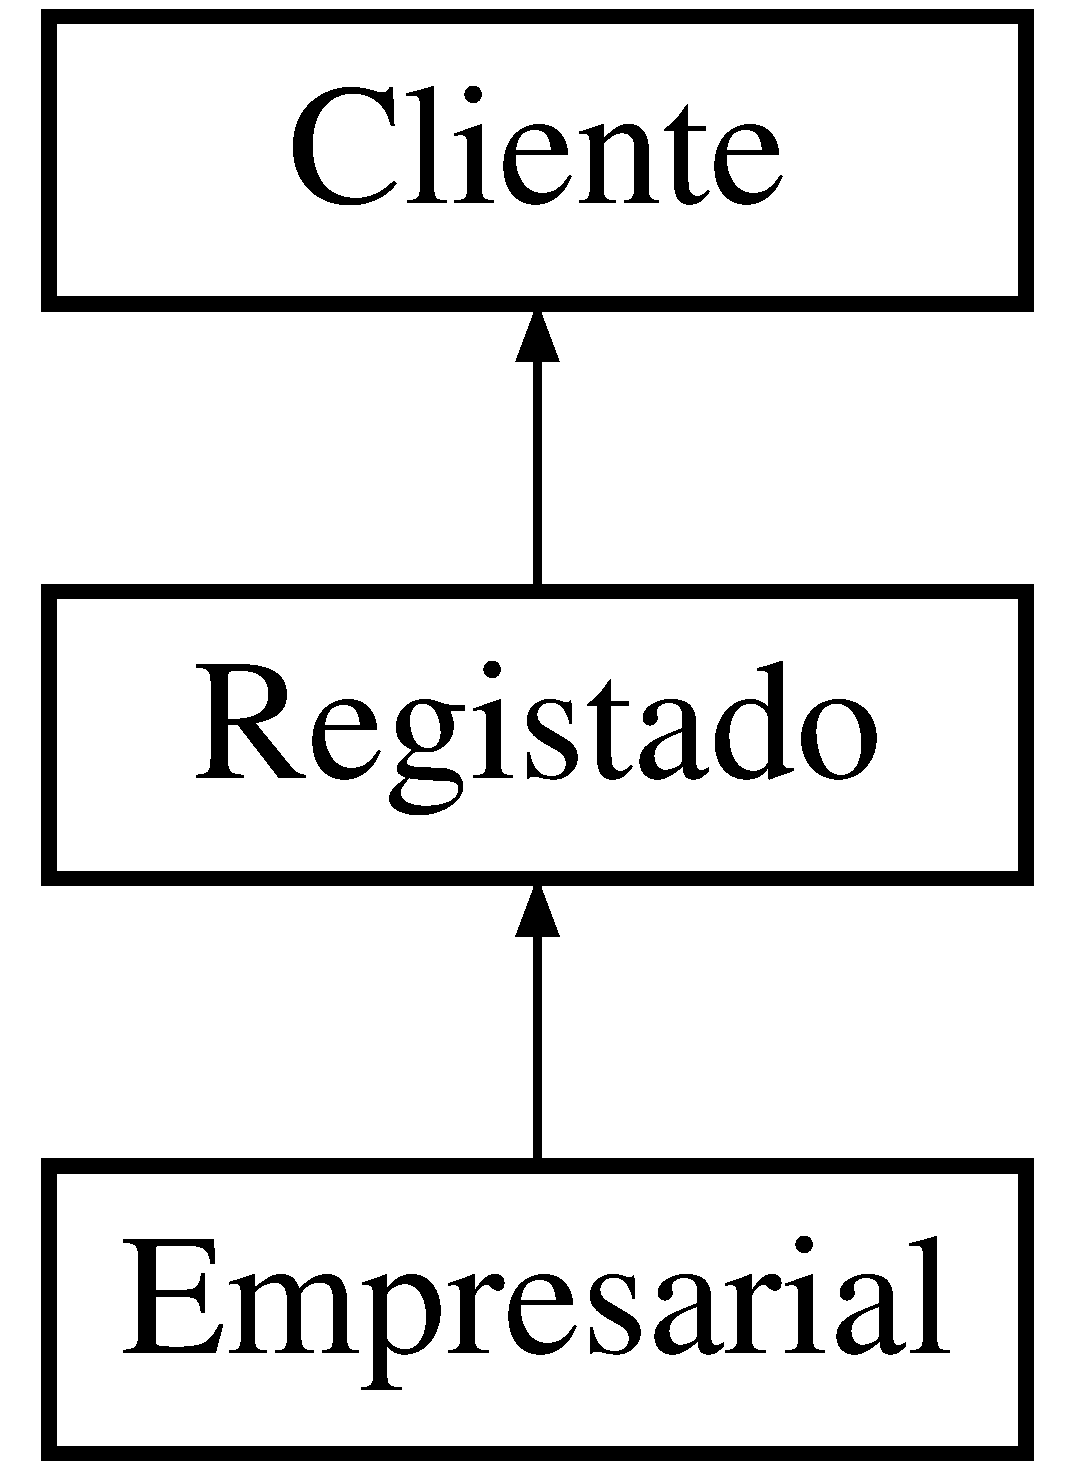
\includegraphics[height=3.000000cm]{class_empresarial}
\end{center}
\end{figure}
\subsection*{Public Member Functions}
\begin{DoxyCompactItemize}
\item 
\hyperlink{class_empresarial_abc2cfe8386b61448ab193977024fe821}{Empresarial} (std\+::string nome, std\+::string morada, const unsigned int N\+IF)
\item 
\hyperlink{class_empresarial_a8f89fe5f36da7bf48548ff67b27e547f}{Empresarial} (std\+::string nome, std\+::string morada)
\item 
\hyperlink{class_empresarial_a1a87eb7f12020af2c8ee8e942f3b8344}{Empresarial} (std\+::string nome)
\item 
virtual std\+::string \hyperlink{class_empresarial_a28090b6b3db16b6b7ba03d6308c2c309}{get\+Informacao} () const
\item 
virtual std\+::string \hyperlink{class_empresarial_a3d5d89f5a446fdcca0955d289592edaf}{get\+Tipo} () const
\end{DoxyCompactItemize}
\subsection*{Additional Inherited Members}


\subsection{Constructor \& Destructor Documentation}
\mbox{\Hypertarget{class_empresarial_abc2cfe8386b61448ab193977024fe821}\label{class_empresarial_abc2cfe8386b61448ab193977024fe821}} 
\index{Empresarial@{Empresarial}!Empresarial@{Empresarial}}
\index{Empresarial@{Empresarial}!Empresarial@{Empresarial}}
\subsubsection{\texorpdfstring{Empresarial()}{Empresarial()}\hspace{0.1cm}{\footnotesize\ttfamily [1/3]}}
{\footnotesize\ttfamily Empresarial\+::\+Empresarial (\begin{DoxyParamCaption}\item[{std\+::string}]{nome,  }\item[{std\+::string}]{morada,  }\item[{const unsigned int}]{N\+IF }\end{DoxyParamCaption})}

Constructor de um cliente \hyperlink{class_empresarial}{Empresarial}, derivado de um cliente \hyperlink{class_registado}{Registado}


\begin{DoxyParams}{Parameters}
{\em nome,morada,int,N\+IF} & \\
\hline
\end{DoxyParams}
\begin{DoxyReturn}{Returns}
bool 
\end{DoxyReturn}
\mbox{\Hypertarget{class_empresarial_a8f89fe5f36da7bf48548ff67b27e547f}\label{class_empresarial_a8f89fe5f36da7bf48548ff67b27e547f}} 
\index{Empresarial@{Empresarial}!Empresarial@{Empresarial}}
\index{Empresarial@{Empresarial}!Empresarial@{Empresarial}}
\subsubsection{\texorpdfstring{Empresarial()}{Empresarial()}\hspace{0.1cm}{\footnotesize\ttfamily [2/3]}}
{\footnotesize\ttfamily Empresarial\+::\+Empresarial (\begin{DoxyParamCaption}\item[{std\+::string}]{nome,  }\item[{std\+::string}]{morada }\end{DoxyParamCaption})}

Constructor de um cliente \hyperlink{class_empresarial}{Empresarial}, derivado de um cliente \hyperlink{class_registado}{Registado}


\begin{DoxyParams}{Parameters}
{\em nome,morada} & \\
\hline
\end{DoxyParams}
\begin{DoxyReturn}{Returns}
bool 
\end{DoxyReturn}
\mbox{\Hypertarget{class_empresarial_a1a87eb7f12020af2c8ee8e942f3b8344}\label{class_empresarial_a1a87eb7f12020af2c8ee8e942f3b8344}} 
\index{Empresarial@{Empresarial}!Empresarial@{Empresarial}}
\index{Empresarial@{Empresarial}!Empresarial@{Empresarial}}
\subsubsection{\texorpdfstring{Empresarial()}{Empresarial()}\hspace{0.1cm}{\footnotesize\ttfamily [3/3]}}
{\footnotesize\ttfamily Empresarial\+::\+Empresarial (\begin{DoxyParamCaption}\item[{std\+::string}]{nome }\end{DoxyParamCaption})}

Constructor de um cliente \hyperlink{class_empresarial}{Empresarial}, derivado de um cliente \hyperlink{class_registado}{Registado}


\begin{DoxyParams}{Parameters}
{\em nome} & \\
\hline
\end{DoxyParams}
\begin{DoxyReturn}{Returns}
bool 
\end{DoxyReturn}


\subsection{Member Function Documentation}
\mbox{\Hypertarget{class_empresarial_a28090b6b3db16b6b7ba03d6308c2c309}\label{class_empresarial_a28090b6b3db16b6b7ba03d6308c2c309}} 
\index{Empresarial@{Empresarial}!get\+Informacao@{get\+Informacao}}
\index{get\+Informacao@{get\+Informacao}!Empresarial@{Empresarial}}
\subsubsection{\texorpdfstring{get\+Informacao()}{getInformacao()}}
{\footnotesize\ttfamily std\+::string Empresarial\+::get\+Informacao (\begin{DoxyParamCaption}{ }\end{DoxyParamCaption}) const\hspace{0.3cm}{\ttfamily [virtual]}}

Obtem informacao de um cliente \hyperlink{class_empresarial}{Empresarial}

\begin{DoxyReturn}{Returns}
string
\end{DoxyReturn}
retorna uma string ja formatda com a informacao relativa a um cliente \hyperlink{class_empresarial}{Empresarial} 

Reimplemented from \hyperlink{class_registado_a7017f0d74afd44459c3d6affcb303d52}{Registado}.

\mbox{\Hypertarget{class_empresarial_a3d5d89f5a446fdcca0955d289592edaf}\label{class_empresarial_a3d5d89f5a446fdcca0955d289592edaf}} 
\index{Empresarial@{Empresarial}!get\+Tipo@{get\+Tipo}}
\index{get\+Tipo@{get\+Tipo}!Empresarial@{Empresarial}}
\subsubsection{\texorpdfstring{get\+Tipo()}{getTipo()}}
{\footnotesize\ttfamily std\+::string Empresarial\+::get\+Tipo (\begin{DoxyParamCaption}{ }\end{DoxyParamCaption}) const\hspace{0.3cm}{\ttfamily [virtual]}}

Constructor de um cliente \hyperlink{class_empresarial}{Empresarial}, derivado de um cliente \hyperlink{class_registado}{Registado}


\begin{DoxyParams}{Parameters}
{\em nome,morada,int,N\+IF} & \\
\hline
\end{DoxyParams}
\begin{DoxyReturn}{Returns}
bool 
\end{DoxyReturn}


Reimplemented from \hyperlink{class_registado}{Registado}.



The documentation for this class was generated from the following files\+:\begin{DoxyCompactItemize}
\item 
C\+:/\+Users/user/\+Desktop/\+Taxis src/src/Cliente.\+h\item 
C\+:/\+Users/user/\+Desktop/\+Taxis src/src/Cliente.\+cpp\end{DoxyCompactItemize}

\hypertarget{class_interface}{}\section{Interface Class Reference}
\label{class_interface}\index{Interface@{Interface}}
\subsection*{Public Member Functions}
\begin{DoxyCompactItemize}
\item 
int \hyperlink{class_interface_ac763e84ad5184ca1eb3886be630b09e3}{Get\+Input} ()
\item 
void \hyperlink{class_interface_afb2590e3e0f91b49c832e3d0f382c376}{Display\+Menu\+Inicial} ()
\item 
void \hyperlink{class_interface_a2b7c19c3b998e017229281c206878d4b}{Menu\+Inicial} (\hyperlink{class_empresa}{Empresa} $\ast$emp)
\item 
void \hyperlink{class_interface_ad35305d21a036b5e7bf6456cc21e9de7}{Display\+Menu\+Principal} ()
\item 
void \hyperlink{class_interface_a480cc121be6baeb6cfd67a3cae133976}{Menu\+Principal} (\hyperlink{class_empresa}{Empresa} $\ast$emp)
\item 
void \hyperlink{class_interface_a14cd6327ea13b33eb29e9529e48edefc}{Novo\+Ficheiro} (\hyperlink{class_empresa}{Empresa} $\ast$emp)
\item 
void \hyperlink{class_interface_a5b714a5d6e7900b9107b473e00d08dae}{Carrega\+Ficheiro} (\hyperlink{class_empresa}{Empresa} $\ast$emp)
\item 
void \hyperlink{class_interface_a3b1b28a27230f16115119c2527e9d8ec}{Guarda\+Ficheiro} (\hyperlink{class_empresa}{Empresa} $\ast$emp)
\item 
\hypertarget{class_interface_a9c40cde97511ef28f13c90542b97a4b3}{}\label{class_interface_a9c40cde97511ef28f13c90542b97a4b3} 
\hyperlink{class_cliente}{Cliente} $\ast$ {\bfseries Criar\+Cliente} ()
\item 
\hyperlink{class_registado}{Registado} $\ast$ \hyperlink{class_interface_afd565930dccaf38d5f9e21efae24ef81}{Criar\+Registado} ()
\item 
\hyperlink{class_servico}{Servico} $\ast$ \hyperlink{class_interface_a5861d0b80a0dde42aa241d1f9281773b}{Criar\+Servico} ()
\item 
\hyperlink{class_empresa}{Empresa} $\ast$ \hyperlink{class_interface_ac7250359ca4316ea76e0c345563e1d16}{Criar\+Empresa} ()
\item 
void \hyperlink{class_interface_adab259ae956337a4d694798e0018c67f}{Display\+Menu\+Pagamento} ()
\item 
void \hyperlink{class_interface_ab5f3406ca0eefdc8a2be60c390a1abe8}{Menu\+Pagamento} (\hyperlink{class_empresa}{Empresa} $\ast$emp)
\end{DoxyCompactItemize}


\subsection{Member Function Documentation}
\hypertarget{class_interface_a5b714a5d6e7900b9107b473e00d08dae}{}\label{class_interface_a5b714a5d6e7900b9107b473e00d08dae} 
\index{Interface@{Interface}!Carrega\+Ficheiro@{Carrega\+Ficheiro}}
\index{Carrega\+Ficheiro@{Carrega\+Ficheiro}!Interface@{Interface}}
\subsubsection{\texorpdfstring{Carrega\+Ficheiro()}{CarregaFicheiro()}}
{\footnotesize\ttfamily void Interface\+::\+Carrega\+Ficheiro (\begin{DoxyParamCaption}\item[{\hyperlink{class_empresa}{Empresa} $\ast$}]{emp }\end{DoxyParamCaption})}

carrega um ficheiro solicitado pelo utilizador para inicio do programa


\begin{DoxyParams}{Parameters}
{\em emp} & \\
\hline
\end{DoxyParams}
\hypertarget{class_interface_ac7250359ca4316ea76e0c345563e1d16}{}\label{class_interface_ac7250359ca4316ea76e0c345563e1d16} 
\index{Interface@{Interface}!Criar\+Empresa@{Criar\+Empresa}}
\index{Criar\+Empresa@{Criar\+Empresa}!Interface@{Interface}}
\subsubsection{\texorpdfstring{Criar\+Empresa()}{CriarEmpresa()}}
{\footnotesize\ttfamily \hyperlink{class_empresa}{Empresa} $\ast$ Interface\+::\+Criar\+Empresa (\begin{DoxyParamCaption}{ }\end{DoxyParamCaption})}

permite ao jogador criar a sua empresa

\begin{DoxyReturn}{Returns}
Empresa$\ast$ 
\end{DoxyReturn}
\hypertarget{class_interface_afd565930dccaf38d5f9e21efae24ef81}{}\label{class_interface_afd565930dccaf38d5f9e21efae24ef81} 
\index{Interface@{Interface}!Criar\+Registado@{Criar\+Registado}}
\index{Criar\+Registado@{Criar\+Registado}!Interface@{Interface}}
\subsubsection{\texorpdfstring{Criar\+Registado()}{CriarRegistado()}}
{\footnotesize\ttfamily \hyperlink{class_registado}{Registado} $\ast$ Interface\+::\+Criar\+Registado (\begin{DoxyParamCaption}{ }\end{DoxyParamCaption})}

�permite ao utilizador criar um cliente \hyperlink{class_registado}{Registado}

\begin{DoxyReturn}{Returns}
Registado$\ast$ 
\end{DoxyReturn}
\hypertarget{class_interface_a5861d0b80a0dde42aa241d1f9281773b}{}\label{class_interface_a5861d0b80a0dde42aa241d1f9281773b} 
\index{Interface@{Interface}!Criar\+Servico@{Criar\+Servico}}
\index{Criar\+Servico@{Criar\+Servico}!Interface@{Interface}}
\subsubsection{\texorpdfstring{Criar\+Servico()}{CriarServico()}}
{\footnotesize\ttfamily \hyperlink{class_servico}{Servico} $\ast$ Interface\+::\+Criar\+Servico (\begin{DoxyParamCaption}{ }\end{DoxyParamCaption})}

permite ao utilizador criar um servico

\begin{DoxyReturn}{Returns}
Servico$\ast$ 
\end{DoxyReturn}
\hypertarget{class_interface_afb2590e3e0f91b49c832e3d0f382c376}{}\label{class_interface_afb2590e3e0f91b49c832e3d0f382c376} 
\index{Interface@{Interface}!Display\+Menu\+Inicial@{Display\+Menu\+Inicial}}
\index{Display\+Menu\+Inicial@{Display\+Menu\+Inicial}!Interface@{Interface}}
\subsubsection{\texorpdfstring{Display\+Menu\+Inicial()}{DisplayMenuInicial()}}
{\footnotesize\ttfamily void Interface\+::\+Display\+Menu\+Inicial (\begin{DoxyParamCaption}{ }\end{DoxyParamCaption})}

mostra o menu inicial \hypertarget{class_interface_adab259ae956337a4d694798e0018c67f}{}\label{class_interface_adab259ae956337a4d694798e0018c67f} 
\index{Interface@{Interface}!Display\+Menu\+Pagamento@{Display\+Menu\+Pagamento}}
\index{Display\+Menu\+Pagamento@{Display\+Menu\+Pagamento}!Interface@{Interface}}
\subsubsection{\texorpdfstring{Display\+Menu\+Pagamento()}{DisplayMenuPagamento()}}
{\footnotesize\ttfamily void Interface\+::\+Display\+Menu\+Pagamento (\begin{DoxyParamCaption}{ }\end{DoxyParamCaption})}

mostra o menu de pagamento \hypertarget{class_interface_ad35305d21a036b5e7bf6456cc21e9de7}{}\label{class_interface_ad35305d21a036b5e7bf6456cc21e9de7} 
\index{Interface@{Interface}!Display\+Menu\+Principal@{Display\+Menu\+Principal}}
\index{Display\+Menu\+Principal@{Display\+Menu\+Principal}!Interface@{Interface}}
\subsubsection{\texorpdfstring{Display\+Menu\+Principal()}{DisplayMenuPrincipal()}}
{\footnotesize\ttfamily void Interface\+::\+Display\+Menu\+Principal (\begin{DoxyParamCaption}{ }\end{DoxyParamCaption})}

mostra o menu principal \hypertarget{class_interface_ac763e84ad5184ca1eb3886be630b09e3}{}\label{class_interface_ac763e84ad5184ca1eb3886be630b09e3} 
\index{Interface@{Interface}!Get\+Input@{Get\+Input}}
\index{Get\+Input@{Get\+Input}!Interface@{Interface}}
\subsubsection{\texorpdfstring{Get\+Input()}{GetInput()}}
{\footnotesize\ttfamily int Interface\+::\+Get\+Input (\begin{DoxyParamCaption}{ }\end{DoxyParamCaption})}

requesita um valor integral ao utilizador

\begin{DoxyReturn}{Returns}
choice 
\end{DoxyReturn}
\hypertarget{class_interface_a3b1b28a27230f16115119c2527e9d8ec}{}\label{class_interface_a3b1b28a27230f16115119c2527e9d8ec} 
\index{Interface@{Interface}!Guarda\+Ficheiro@{Guarda\+Ficheiro}}
\index{Guarda\+Ficheiro@{Guarda\+Ficheiro}!Interface@{Interface}}
\subsubsection{\texorpdfstring{Guarda\+Ficheiro()}{GuardaFicheiro()}}
{\footnotesize\ttfamily void Interface\+::\+Guarda\+Ficheiro (\begin{DoxyParamCaption}\item[{\hyperlink{class_empresa}{Empresa} $\ast$}]{emp }\end{DoxyParamCaption})}

guarda a sessao actual num ficheiro solicitado pelo utilizador


\begin{DoxyParams}{Parameters}
{\em emp} & \\
\hline
\end{DoxyParams}
\hypertarget{class_interface_a2b7c19c3b998e017229281c206878d4b}{}\label{class_interface_a2b7c19c3b998e017229281c206878d4b} 
\index{Interface@{Interface}!Menu\+Inicial@{Menu\+Inicial}}
\index{Menu\+Inicial@{Menu\+Inicial}!Interface@{Interface}}
\subsubsection{\texorpdfstring{Menu\+Inicial()}{MenuInicial()}}
{\footnotesize\ttfamily void Interface\+::\+Menu\+Inicial (\begin{DoxyParamCaption}\item[{\hyperlink{class_empresa}{Empresa} $\ast$}]{emp }\end{DoxyParamCaption})}

invoca o menu inicial e a sua logica


\begin{DoxyParams}{Parameters}
{\em emp} & \\
\hline
\end{DoxyParams}
\hypertarget{class_interface_ab5f3406ca0eefdc8a2be60c390a1abe8}{}\label{class_interface_ab5f3406ca0eefdc8a2be60c390a1abe8} 
\index{Interface@{Interface}!Menu\+Pagamento@{Menu\+Pagamento}}
\index{Menu\+Pagamento@{Menu\+Pagamento}!Interface@{Interface}}
\subsubsection{\texorpdfstring{Menu\+Pagamento()}{MenuPagamento()}}
{\footnotesize\ttfamily void Interface\+::\+Menu\+Pagamento (\begin{DoxyParamCaption}\item[{\hyperlink{class_empresa}{Empresa} $\ast$}]{emp }\end{DoxyParamCaption})}

invoca o menu de pagamento e a sua logica


\begin{DoxyParams}{Parameters}
{\em emp} & \\
\hline
\end{DoxyParams}
\hypertarget{class_interface_a480cc121be6baeb6cfd67a3cae133976}{}\label{class_interface_a480cc121be6baeb6cfd67a3cae133976} 
\index{Interface@{Interface}!Menu\+Principal@{Menu\+Principal}}
\index{Menu\+Principal@{Menu\+Principal}!Interface@{Interface}}
\subsubsection{\texorpdfstring{Menu\+Principal()}{MenuPrincipal()}}
{\footnotesize\ttfamily void Interface\+::\+Menu\+Principal (\begin{DoxyParamCaption}\item[{\hyperlink{class_empresa}{Empresa} $\ast$}]{emp }\end{DoxyParamCaption})}

invoca o menu principal e a sua logica


\begin{DoxyParams}{Parameters}
{\em emp} & \\
\hline
\end{DoxyParams}
\hypertarget{class_interface_a14cd6327ea13b33eb29e9529e48edefc}{}\label{class_interface_a14cd6327ea13b33eb29e9529e48edefc} 
\index{Interface@{Interface}!Novo\+Ficheiro@{Novo\+Ficheiro}}
\index{Novo\+Ficheiro@{Novo\+Ficheiro}!Interface@{Interface}}
\subsubsection{\texorpdfstring{Novo\+Ficheiro()}{NovoFicheiro()}}
{\footnotesize\ttfamily void Interface\+::\+Novo\+Ficheiro (\begin{DoxyParamCaption}\item[{\hyperlink{class_empresa}{Empresa} $\ast$}]{emp }\end{DoxyParamCaption})}

solicita a criacao de um novo ficheiro para o inicio do programam


\begin{DoxyParams}{Parameters}
{\em emp} & \\
\hline
\end{DoxyParams}


The documentation for this class was generated from the following files\+:\begin{DoxyCompactItemize}
\item 
C\+:/\+Users/\+User\+Candido/\+Desktop/\+Eclipse A\+E\+D\+A/\+C\+A\+L/\+Taxis 2/src/Interface.\+h\item 
C\+:/\+Users/\+User\+Candido/\+Desktop/\+Eclipse A\+E\+D\+A/\+C\+A\+L/\+Taxis 2/src/Interface.\+cpp\end{DoxyCompactItemize}

\hypertarget{class_particular}{}\section{Particular Class Reference}
\label{class_particular}\index{Particular@{Particular}}
Inheritance diagram for Particular\+:\begin{figure}[H]
\begin{center}
\leavevmode
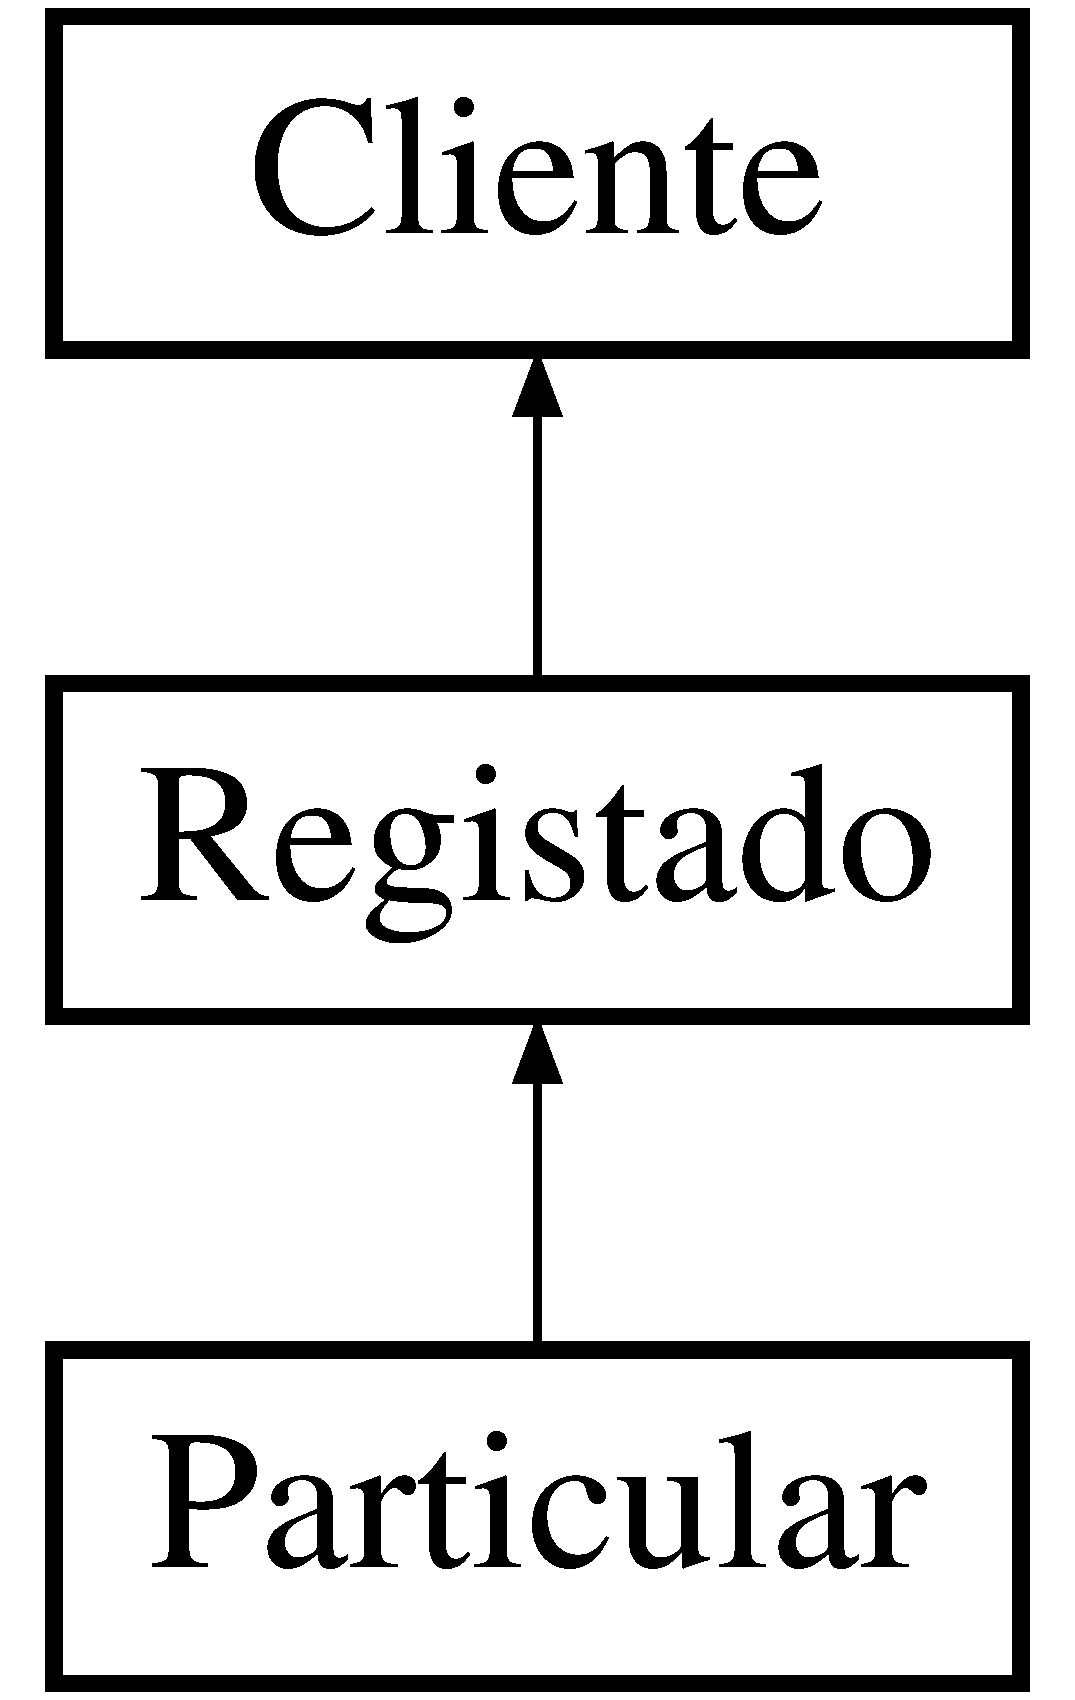
\includegraphics[height=3.000000cm]{class_particular}
\end{center}
\end{figure}
\subsection*{Public Member Functions}
\begin{DoxyCompactItemize}
\item 
\hyperlink{class_particular_a355034b30f29b3fecf6654de8d652aa7}{Particular} (std\+::string nome, std\+::string morada, const unsigned int N\+IF)
\item 
\hyperlink{class_particular_a794314799e022e8f05fda84af1722bc8}{Particular} (std\+::string nome, std\+::string morada)
\item 
\hyperlink{class_particular_a55ebdb7b32d55be44f903be5a4f4d6aa}{Particular} (std\+::string nome)
\item 
virtual std\+::string \hyperlink{class_particular_acde85dcb3d26ca3afe131fb4c35763c8}{get\+Informacao} () const
\item 
virtual std\+::string \hyperlink{class_particular_ac7fc22a792b8c711d5f424ad9af19755}{get\+Tipo} () const
\end{DoxyCompactItemize}
\subsection*{Additional Inherited Members}


\subsection{Constructor \& Destructor Documentation}
\hypertarget{class_particular_a355034b30f29b3fecf6654de8d652aa7}{}\label{class_particular_a355034b30f29b3fecf6654de8d652aa7} 
\index{Particular@{Particular}!Particular@{Particular}}
\index{Particular@{Particular}!Particular@{Particular}}
\subsubsection{\texorpdfstring{Particular()}{Particular()}\hspace{0.1cm}{\footnotesize\ttfamily [1/3]}}
{\footnotesize\ttfamily Particular\+::\+Particular (\begin{DoxyParamCaption}\item[{std\+::string}]{nome,  }\item[{std\+::string}]{morada,  }\item[{const unsigned int}]{N\+IF }\end{DoxyParamCaption})}

Constructor de um cliente \hyperlink{class_particular}{Particular}, derivado de um cliente \hyperlink{class_registado}{Registado}


\begin{DoxyParams}{Parameters}
{\em nome,morada,int,N\+IF} & \\
\hline
\end{DoxyParams}
\begin{DoxyReturn}{Returns}
bool 
\end{DoxyReturn}
\hypertarget{class_particular_a794314799e022e8f05fda84af1722bc8}{}\label{class_particular_a794314799e022e8f05fda84af1722bc8} 
\index{Particular@{Particular}!Particular@{Particular}}
\index{Particular@{Particular}!Particular@{Particular}}
\subsubsection{\texorpdfstring{Particular()}{Particular()}\hspace{0.1cm}{\footnotesize\ttfamily [2/3]}}
{\footnotesize\ttfamily Particular\+::\+Particular (\begin{DoxyParamCaption}\item[{std\+::string}]{nome,  }\item[{std\+::string}]{morada }\end{DoxyParamCaption})}

Constructor de um cliente \hyperlink{class_particular}{Particular}, derivado de um cliente \hyperlink{class_registado}{Registado}


\begin{DoxyParams}{Parameters}
{\em nome,morada,int} & \\
\hline
\end{DoxyParams}
\hypertarget{class_particular_a55ebdb7b32d55be44f903be5a4f4d6aa}{}\label{class_particular_a55ebdb7b32d55be44f903be5a4f4d6aa} 
\index{Particular@{Particular}!Particular@{Particular}}
\index{Particular@{Particular}!Particular@{Particular}}
\subsubsection{\texorpdfstring{Particular()}{Particular()}\hspace{0.1cm}{\footnotesize\ttfamily [3/3]}}
{\footnotesize\ttfamily Particular\+::\+Particular (\begin{DoxyParamCaption}\item[{std\+::string}]{nome }\end{DoxyParamCaption})}

Constructor de um cliente \hyperlink{class_particular}{Particular}, derivado de um cliente \hyperlink{class_registado}{Registado}


\begin{DoxyParams}{Parameters}
{\em nome} & \\
\hline
\end{DoxyParams}


\subsection{Member Function Documentation}
\hypertarget{class_particular_acde85dcb3d26ca3afe131fb4c35763c8}{}\label{class_particular_acde85dcb3d26ca3afe131fb4c35763c8} 
\index{Particular@{Particular}!get\+Informacao@{get\+Informacao}}
\index{get\+Informacao@{get\+Informacao}!Particular@{Particular}}
\subsubsection{\texorpdfstring{get\+Informacao()}{getInformacao()}}
{\footnotesize\ttfamily std\+::string Particular\+::get\+Informacao (\begin{DoxyParamCaption}{ }\end{DoxyParamCaption}) const\hspace{0.3cm}{\ttfamily [virtual]}}

Obtem informacao relativa a um cliente \hyperlink{class_particular}{Particular}

\begin{DoxyReturn}{Returns}
string
\end{DoxyReturn}
retorna uma string ja formatada com a informaca relativa a um cliente particular 

Reimplemented from \hyperlink{class_registado_a7017f0d74afd44459c3d6affcb303d52}{Registado}.

\hypertarget{class_particular_ac7fc22a792b8c711d5f424ad9af19755}{}\label{class_particular_ac7fc22a792b8c711d5f424ad9af19755} 
\index{Particular@{Particular}!get\+Tipo@{get\+Tipo}}
\index{get\+Tipo@{get\+Tipo}!Particular@{Particular}}
\subsubsection{\texorpdfstring{get\+Tipo()}{getTipo()}}
{\footnotesize\ttfamily std\+::string Particular\+::get\+Tipo (\begin{DoxyParamCaption}{ }\end{DoxyParamCaption}) const\hspace{0.3cm}{\ttfamily [virtual]}}

Constructor de um cliente \hyperlink{class_particular}{Particular}, derivado de um cliente \hyperlink{class_registado}{Registado}

\begin{DoxyReturn}{Returns}
string
\end{DoxyReturn}
retorna uma string que representao o tipo de cliente (particular ou empresarial) de um cliente \hyperlink{class_registado}{Registado} 

Reimplemented from \hyperlink{class_registado}{Registado}.



The documentation for this class was generated from the following files\+:\begin{DoxyCompactItemize}
\item 
C\+:/\+Users/\+User\+Candido/\+Desktop/\+Eclipse A\+E\+D\+A/\+C\+A\+L/\+Taxis 2/src/Cliente.\+h\item 
C\+:/\+Users/\+User\+Candido/\+Desktop/\+Eclipse A\+E\+D\+A/\+C\+A\+L/\+Taxis 2/src/Cliente.\+cpp\end{DoxyCompactItemize}

\hypertarget{class_registado}{}\section{Registado Class Reference}
\label{class_registado}\index{Registado@{Registado}}
Inheritance diagram for Registado\+:\begin{figure}[H]
\begin{center}
\leavevmode
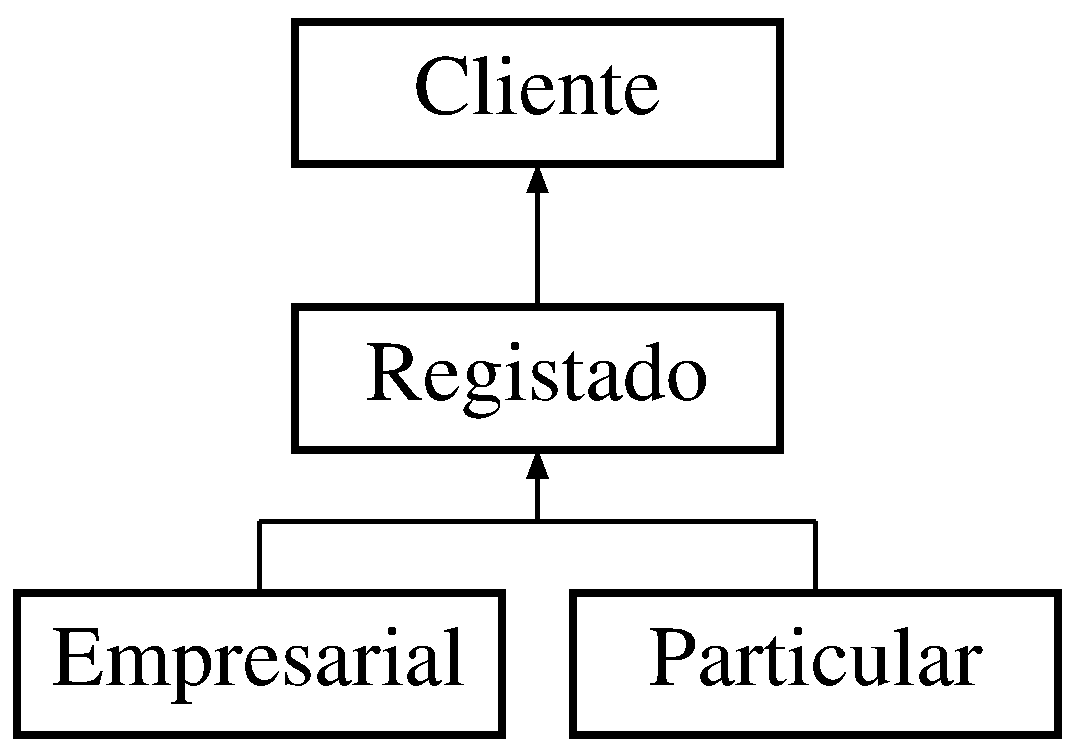
\includegraphics[height=3.000000cm]{class_registado}
\end{center}
\end{figure}
\subsection*{Public Member Functions}
\begin{DoxyCompactItemize}
\item 
\hyperlink{class_registado_ace8988ba72da772309e5aebf0bc82d4d}{Registado} (std\+::string nome, std\+::string morada, const unsigned int N\+IF)
\item 
\hyperlink{class_registado_a2ebad03ff43e207581c62952a88129b4}{Registado} (std\+::string nome, std\+::string morada)
\item 
\hyperlink{class_registado_a67a8d0c0dbd3103deae8813eb0958752}{Registado} (std\+::string nome)
\item 
std\+::vector$<$ \hyperlink{class_servico}{Servico} $\ast$ $>$ \hyperlink{class_registado_a304848f6ce1d82ad8438ec5e273cbc2d}{get\+Historico} () const
\item 
virtual std\+::string \hyperlink{class_registado_a7017f0d74afd44459c3d6affcb303d52}{get\+Informacao} () const
\item 
void \hyperlink{class_registado_a4570e0b507ef86f7fce56510f118a887}{operator=} (const \hyperlink{class_registado}{Registado} \&reg)
\item 
virtual std\+::string \hyperlink{class_registado_a15109adc7cd6a8834bd2ef909bcde008}{get\+Informacao\+Servicos} () const
\item 
\hypertarget{class_registado_a3512b905e10ee9a629c4dbbdc692f420}{}\label{class_registado_a3512b905e10ee9a629c4dbbdc692f420} 
virtual std\+::string {\bfseries get\+Tipo} () const
\item 
virtual bool \hyperlink{class_registado_af3c8f63f7df1cdfd27e44126f78b71d8}{pagamento\+Numerario} (\hyperlink{class_servico}{Servico} \&serv)
\item 
virtual bool \hyperlink{class_registado_a36be4ccf8e4b1bc26be7c1c2d4612229}{pagamento\+Multibanco} (\hyperlink{class_servico}{Servico} \&serv)
\item 
virtual bool \hyperlink{class_registado_a1d6da4b2cbc8340fa79055a026d4ea44}{pagamento\+Cartao\+Credito} (\hyperlink{class_servico}{Servico} \&serv)
\item 
virtual bool \hyperlink{class_registado_a87218f9b1e1aa767c6c77b71f38cca55}{pagamento\+Fim\+Do\+Mes} (std\+::vector$<$ \hyperlink{class_servico}{Servico} $\ast$$>$ servs)
\item 
virtual bool \hyperlink{class_registado_a16a6ec63ed53fd4b6ebb1105ae5812d7}{pagamento\+Numerario} (unsigned int id)
\item 
virtual bool \hyperlink{class_registado_a3338ad6a9c5980671f2eb3b48d8798de}{pagamento\+Multibanco} (unsigned int id)
\item 
virtual bool \hyperlink{class_registado_a957b62d73c6ea619fb29e63255e11b12}{pagamento\+Cartao\+Credito} (unsigned int id)
\item 
virtual bool \hyperlink{class_registado_a0ee7364d85601f95bfe6bf45c062ec06}{pagamento\+Fim\+Do\+Mes} (std\+::vector$<$ unsigned int $>$ ids)
\item 
bool \hyperlink{class_registado_acc2088074502804017ff3e40022d966c}{adiciona\+Servico} (\hyperlink{class_servico}{Servico} $\ast$serv)
\end{DoxyCompactItemize}
\subsection*{Private Attributes}
\begin{DoxyCompactItemize}
\item 
\hypertarget{class_registado_ab5a4890cf0db0c42da0caeecb6f9f31f}{}\label{class_registado_ab5a4890cf0db0c42da0caeecb6f9f31f} 
std\+::vector$<$ \hyperlink{class_servico}{Servico} $\ast$ $>$ {\bfseries historico}
\end{DoxyCompactItemize}
\subsection*{Additional Inherited Members}


\subsection{Constructor \& Destructor Documentation}
\hypertarget{class_registado_ace8988ba72da772309e5aebf0bc82d4d}{}\label{class_registado_ace8988ba72da772309e5aebf0bc82d4d} 
\index{Registado@{Registado}!Registado@{Registado}}
\index{Registado@{Registado}!Registado@{Registado}}
\subsubsection{\texorpdfstring{Registado()}{Registado()}\hspace{0.1cm}{\footnotesize\ttfamily [1/3]}}
{\footnotesize\ttfamily Registado\+::\+Registado (\begin{DoxyParamCaption}\item[{std\+::string}]{nome,  }\item[{std\+::string}]{morada,  }\item[{const unsigned int}]{N\+IF }\end{DoxyParamCaption})}


\begin{DoxyParams}{Parameters}
{\em nome,morada,N\+IF} & constructor da classe \hyperlink{class_registado}{Registado}, derivadaa da classe \hyperlink{class_cliente}{Cliente} \\
\hline
\end{DoxyParams}
\hypertarget{class_registado_a2ebad03ff43e207581c62952a88129b4}{}\label{class_registado_a2ebad03ff43e207581c62952a88129b4} 
\index{Registado@{Registado}!Registado@{Registado}}
\index{Registado@{Registado}!Registado@{Registado}}
\subsubsection{\texorpdfstring{Registado()}{Registado()}\hspace{0.1cm}{\footnotesize\ttfamily [2/3]}}
{\footnotesize\ttfamily Registado\+::\+Registado (\begin{DoxyParamCaption}\item[{std\+::string}]{nome,  }\item[{std\+::string}]{morada }\end{DoxyParamCaption})}

Constructor de \hyperlink{class_registado}{Registado} 
\begin{DoxyParams}{Parameters}
{\em nome,morada,N\+IF} & \\
\hline
\end{DoxyParams}
\hypertarget{class_registado_a67a8d0c0dbd3103deae8813eb0958752}{}\label{class_registado_a67a8d0c0dbd3103deae8813eb0958752} 
\index{Registado@{Registado}!Registado@{Registado}}
\index{Registado@{Registado}!Registado@{Registado}}
\subsubsection{\texorpdfstring{Registado()}{Registado()}\hspace{0.1cm}{\footnotesize\ttfamily [3/3]}}
{\footnotesize\ttfamily Registado\+::\+Registado (\begin{DoxyParamCaption}\item[{std\+::string}]{nome }\end{DoxyParamCaption})}


\begin{DoxyParams}{Parameters}
{\em nome} & Constructor de um cliente \hyperlink{class_registado}{Registado} \\
\hline
\end{DoxyParams}


\subsection{Member Function Documentation}
\hypertarget{class_registado_acc2088074502804017ff3e40022d966c}{}\label{class_registado_acc2088074502804017ff3e40022d966c} 
\index{Registado@{Registado}!adiciona\+Servico@{adiciona\+Servico}}
\index{adiciona\+Servico@{adiciona\+Servico}!Registado@{Registado}}
\subsubsection{\texorpdfstring{adiciona\+Servico()}{adicionaServico()}}
{\footnotesize\ttfamily bool Registado\+::adiciona\+Servico (\begin{DoxyParamCaption}\item[{\hyperlink{class_servico}{Servico} $\ast$}]{serv }\end{DoxyParamCaption})}

Adiciona um \hyperlink{class_servico}{Servico} a um cliente \hyperlink{class_registado}{Registado}


\begin{DoxyParams}{Parameters}
{\em serv} & \\
\hline
\end{DoxyParams}
\begin{DoxyReturn}{Returns}
bool
\end{DoxyReturn}
adiciona, se possivel, um servico ao historico de servicos de um cliente registado \hypertarget{class_registado_a304848f6ce1d82ad8438ec5e273cbc2d}{}\label{class_registado_a304848f6ce1d82ad8438ec5e273cbc2d} 
\index{Registado@{Registado}!get\+Historico@{get\+Historico}}
\index{get\+Historico@{get\+Historico}!Registado@{Registado}}
\subsubsection{\texorpdfstring{get\+Historico()}{getHistorico()}}
{\footnotesize\ttfamily std\+::vector$<$ \hyperlink{class_servico}{Servico} $\ast$ $>$ Registado\+::get\+Historico (\begin{DoxyParamCaption}{ }\end{DoxyParamCaption}) const}

\begin{DoxyReturn}{Returns}
historico
\end{DoxyReturn}
retorna o historico de clientes requesitados de um cliente registado \hypertarget{class_registado_a7017f0d74afd44459c3d6affcb303d52}{}\label{class_registado_a7017f0d74afd44459c3d6affcb303d52} 
\index{Registado@{Registado}!get\+Informacao@{get\+Informacao}}
\index{get\+Informacao@{get\+Informacao}!Registado@{Registado}}
\subsubsection{\texorpdfstring{get\+Informacao()}{getInformacao()}}
{\footnotesize\ttfamily std\+::string Registado\+::get\+Informacao (\begin{DoxyParamCaption}{ }\end{DoxyParamCaption}) const\hspace{0.3cm}{\ttfamily [virtual]}}

Informacao sobre um cliente \hyperlink{class_registado}{Registado}


\begin{DoxyParams}{Parameters}
{\em string} & retorna uma string com a informacao ja formatada relativamente a um cliente \hyperlink{class_registado}{Registado} \\
\hline
\end{DoxyParams}


Reimplemented from \hyperlink{class_cliente_a932ef71b2792dc5df153f82d3e81a6f3}{Cliente}.



Reimplemented in \hyperlink{class_particular_acde85dcb3d26ca3afe131fb4c35763c8}{Particular}, and \hyperlink{class_empresarial_a28090b6b3db16b6b7ba03d6308c2c309}{Empresarial}.

\hypertarget{class_registado_a15109adc7cd6a8834bd2ef909bcde008}{}\label{class_registado_a15109adc7cd6a8834bd2ef909bcde008} 
\index{Registado@{Registado}!get\+Informacao\+Servicos@{get\+Informacao\+Servicos}}
\index{get\+Informacao\+Servicos@{get\+Informacao\+Servicos}!Registado@{Registado}}
\subsubsection{\texorpdfstring{get\+Informacao\+Servicos()}{getInformacaoServicos()}}
{\footnotesize\ttfamily std\+::string Registado\+::get\+Informacao\+Servicos (\begin{DoxyParamCaption}{ }\end{DoxyParamCaption}) const\hspace{0.3cm}{\ttfamily [virtual]}}

Informacao relativa a sericos

\begin{DoxyReturn}{Returns}
string
\end{DoxyReturn}
Retorna uma string ja formatada com a informacao relativa aos servicos todos do historico de um cliente \hypertarget{class_registado_a4570e0b507ef86f7fce56510f118a887}{}\label{class_registado_a4570e0b507ef86f7fce56510f118a887} 
\index{Registado@{Registado}!operator=@{operator=}}
\index{operator=@{operator=}!Registado@{Registado}}
\subsubsection{\texorpdfstring{operator=()}{operator=()}}
{\footnotesize\ttfamily void Registado\+::operator= (\begin{DoxyParamCaption}\item[{const \hyperlink{class_registado}{Registado} \&}]{reg }\end{DoxyParamCaption})}

Operador = para a classe \hyperlink{class_registado}{Registado}, derivado da classe \hyperlink{class_cliente}{Cliente} 
\begin{DoxyParams}{Parameters}
{\em reg} & \\
\hline
\end{DoxyParams}
iguala o nome, morada, N\+IF e historico (historico de servicos requesitados do cliente registado) aos membros equivalentes de outro cliente registado \hypertarget{class_registado_a1d6da4b2cbc8340fa79055a026d4ea44}{}\label{class_registado_a1d6da4b2cbc8340fa79055a026d4ea44} 
\index{Registado@{Registado}!pagamento\+Cartao\+Credito@{pagamento\+Cartao\+Credito}}
\index{pagamento\+Cartao\+Credito@{pagamento\+Cartao\+Credito}!Registado@{Registado}}
\subsubsection{\texorpdfstring{pagamento\+Cartao\+Credito()}{pagamentoCartaoCredito()}\hspace{0.1cm}{\footnotesize\ttfamily [1/2]}}
{\footnotesize\ttfamily bool Registado\+::pagamento\+Cartao\+Credito (\begin{DoxyParamCaption}\item[{\hyperlink{class_servico}{Servico} \&}]{serv }\end{DoxyParamCaption})\hspace{0.3cm}{\ttfamily [virtual]}}

Pagamento de um \hyperlink{class_servico}{Servico} de um cliente \hyperlink{class_registado}{Registado}


\begin{DoxyParams}{Parameters}
{\em serv} & \\
\hline
\end{DoxyParams}
\begin{DoxyReturn}{Returns}
bool
\end{DoxyReturn}
efectua o pagamento de um servico a um cliente \hyperlink{class_registado}{Registado} segundo o metodo de pagamento por cartao de credito \hypertarget{class_registado_a957b62d73c6ea619fb29e63255e11b12}{}\label{class_registado_a957b62d73c6ea619fb29e63255e11b12} 
\index{Registado@{Registado}!pagamento\+Cartao\+Credito@{pagamento\+Cartao\+Credito}}
\index{pagamento\+Cartao\+Credito@{pagamento\+Cartao\+Credito}!Registado@{Registado}}
\subsubsection{\texorpdfstring{pagamento\+Cartao\+Credito()}{pagamentoCartaoCredito()}\hspace{0.1cm}{\footnotesize\ttfamily [2/2]}}
{\footnotesize\ttfamily bool Registado\+::pagamento\+Cartao\+Credito (\begin{DoxyParamCaption}\item[{unsigned int}]{id }\end{DoxyParamCaption})\hspace{0.3cm}{\ttfamily [virtual]}}

Pagamento de um \hyperlink{class_servico}{Servico} de um cliente \hyperlink{class_registado}{Registado}


\begin{DoxyParams}{Parameters}
{\em id} & \\
\hline
\end{DoxyParams}
\begin{DoxyReturn}{Returns}
bool
\end{DoxyReturn}
efectua o pagamento de um servico a um cliente \hyperlink{class_registado}{Registado} segundo o metodo de pagamento por cartao de credito \hypertarget{class_registado_a87218f9b1e1aa767c6c77b71f38cca55}{}\label{class_registado_a87218f9b1e1aa767c6c77b71f38cca55} 
\index{Registado@{Registado}!pagamento\+Fim\+Do\+Mes@{pagamento\+Fim\+Do\+Mes}}
\index{pagamento\+Fim\+Do\+Mes@{pagamento\+Fim\+Do\+Mes}!Registado@{Registado}}
\subsubsection{\texorpdfstring{pagamento\+Fim\+Do\+Mes()}{pagamentoFimDoMes()}\hspace{0.1cm}{\footnotesize\ttfamily [1/2]}}
{\footnotesize\ttfamily bool Registado\+::pagamento\+Fim\+Do\+Mes (\begin{DoxyParamCaption}\item[{std\+::vector$<$ \hyperlink{class_servico}{Servico} $\ast$$>$}]{servs }\end{DoxyParamCaption})\hspace{0.3cm}{\ttfamily [virtual]}}

Pagamento de um \hyperlink{class_servico}{Servico} de um cliente \hyperlink{class_registado}{Registado}


\begin{DoxyParams}{Parameters}
{\em servs} & \\
\hline
\end{DoxyParams}
\begin{DoxyReturn}{Returns}
bool
\end{DoxyReturn}
efectua o pagamento dos servicos de um vector de servicos (historico) a um cliente \hyperlink{class_registado}{Registado} segundo o metodo de pagamento ao fim do mes \hypertarget{class_registado_a0ee7364d85601f95bfe6bf45c062ec06}{}\label{class_registado_a0ee7364d85601f95bfe6bf45c062ec06} 
\index{Registado@{Registado}!pagamento\+Fim\+Do\+Mes@{pagamento\+Fim\+Do\+Mes}}
\index{pagamento\+Fim\+Do\+Mes@{pagamento\+Fim\+Do\+Mes}!Registado@{Registado}}
\subsubsection{\texorpdfstring{pagamento\+Fim\+Do\+Mes()}{pagamentoFimDoMes()}\hspace{0.1cm}{\footnotesize\ttfamily [2/2]}}
{\footnotesize\ttfamily bool Registado\+::pagamento\+Fim\+Do\+Mes (\begin{DoxyParamCaption}\item[{std\+::vector$<$ unsigned int $>$}]{ids }\end{DoxyParamCaption})\hspace{0.3cm}{\ttfamily [virtual]}}

Pagamento de um \hyperlink{class_servico}{Servico} de um cliente \hyperlink{class_registado}{Registado}


\begin{DoxyParams}{Parameters}
{\em ids} & \\
\hline
\end{DoxyParams}
\begin{DoxyReturn}{Returns}
bool
\end{DoxyReturn}
efectua o pagamento de um vector de ids de servicos a um cliente \hyperlink{class_registado}{Registado} segundo o metodo de pagamento ao fim do mes \hypertarget{class_registado_a36be4ccf8e4b1bc26be7c1c2d4612229}{}\label{class_registado_a36be4ccf8e4b1bc26be7c1c2d4612229} 
\index{Registado@{Registado}!pagamento\+Multibanco@{pagamento\+Multibanco}}
\index{pagamento\+Multibanco@{pagamento\+Multibanco}!Registado@{Registado}}
\subsubsection{\texorpdfstring{pagamento\+Multibanco()}{pagamentoMultibanco()}\hspace{0.1cm}{\footnotesize\ttfamily [1/2]}}
{\footnotesize\ttfamily bool Registado\+::pagamento\+Multibanco (\begin{DoxyParamCaption}\item[{\hyperlink{class_servico}{Servico} \&}]{serv }\end{DoxyParamCaption})\hspace{0.3cm}{\ttfamily [virtual]}}

Pagamento de um \hyperlink{class_servico}{Servico} de um cliente \hyperlink{class_registado}{Registado}


\begin{DoxyParams}{Parameters}
{\em serv} & \\
\hline
\end{DoxyParams}
\begin{DoxyReturn}{Returns}
bool
\end{DoxyReturn}
efectua o pagamento de um servico a um cliente \hyperlink{class_registado}{Registado} segundo o metodo de pagamento por multibanco 

Reimplemented from \hyperlink{class_cliente_a6e230e5e512bebe07bfa1ad6750b8cee}{Cliente}.

\hypertarget{class_registado_a3338ad6a9c5980671f2eb3b48d8798de}{}\label{class_registado_a3338ad6a9c5980671f2eb3b48d8798de} 
\index{Registado@{Registado}!pagamento\+Multibanco@{pagamento\+Multibanco}}
\index{pagamento\+Multibanco@{pagamento\+Multibanco}!Registado@{Registado}}
\subsubsection{\texorpdfstring{pagamento\+Multibanco()}{pagamentoMultibanco()}\hspace{0.1cm}{\footnotesize\ttfamily [2/2]}}
{\footnotesize\ttfamily bool Registado\+::pagamento\+Multibanco (\begin{DoxyParamCaption}\item[{unsigned int}]{id }\end{DoxyParamCaption})\hspace{0.3cm}{\ttfamily [virtual]}}

Pagamento de um \hyperlink{class_servico}{Servico} de um cliente \hyperlink{class_registado}{Registado}


\begin{DoxyParams}{Parameters}
{\em id} & \\
\hline
\end{DoxyParams}
\begin{DoxyReturn}{Returns}
bool
\end{DoxyReturn}
efectua o pagamento de um servico a um cliente \hyperlink{class_registado}{Registado} segundo o metodo de pagamento por multibanco \hypertarget{class_registado_af3c8f63f7df1cdfd27e44126f78b71d8}{}\label{class_registado_af3c8f63f7df1cdfd27e44126f78b71d8} 
\index{Registado@{Registado}!pagamento\+Numerario@{pagamento\+Numerario}}
\index{pagamento\+Numerario@{pagamento\+Numerario}!Registado@{Registado}}
\subsubsection{\texorpdfstring{pagamento\+Numerario()}{pagamentoNumerario()}\hspace{0.1cm}{\footnotesize\ttfamily [1/2]}}
{\footnotesize\ttfamily bool Registado\+::pagamento\+Numerario (\begin{DoxyParamCaption}\item[{\hyperlink{class_servico}{Servico} \&}]{serv }\end{DoxyParamCaption})\hspace{0.3cm}{\ttfamily [virtual]}}

Pagamento de um \hyperlink{class_servico}{Servico} de um cliente \hyperlink{class_registado}{Registado}


\begin{DoxyParams}{Parameters}
{\em serv} & \\
\hline
\end{DoxyParams}
\begin{DoxyReturn}{Returns}
bool
\end{DoxyReturn}
efectua o pagamento de um servico a um cliente \hyperlink{class_registado}{Registado} segundo o metodo de pagamento por numerario 

Reimplemented from \hyperlink{class_cliente_a68646846a80de5cdcb61b1f8a13e4fb8}{Cliente}.

\hypertarget{class_registado_a16a6ec63ed53fd4b6ebb1105ae5812d7}{}\label{class_registado_a16a6ec63ed53fd4b6ebb1105ae5812d7} 
\index{Registado@{Registado}!pagamento\+Numerario@{pagamento\+Numerario}}
\index{pagamento\+Numerario@{pagamento\+Numerario}!Registado@{Registado}}
\subsubsection{\texorpdfstring{pagamento\+Numerario()}{pagamentoNumerario()}\hspace{0.1cm}{\footnotesize\ttfamily [2/2]}}
{\footnotesize\ttfamily bool Registado\+::pagamento\+Numerario (\begin{DoxyParamCaption}\item[{unsigned int}]{id }\end{DoxyParamCaption})\hspace{0.3cm}{\ttfamily [virtual]}}

Pagamento de um \hyperlink{class_servico}{Servico} de um cliente \hyperlink{class_registado}{Registado}


\begin{DoxyParams}{Parameters}
{\em id} & \\
\hline
\end{DoxyParams}
\begin{DoxyReturn}{Returns}
bool
\end{DoxyReturn}
efectua o pagamento de um servico a um cliente \hyperlink{class_registado}{Registado} segundo o metodo de pagamento por numerario 

The documentation for this class was generated from the following files\+:\begin{DoxyCompactItemize}
\item 
C\+:/\+Users/\+User\+Candido/\+Desktop/\+Eclipse A\+E\+D\+A/\+C\+A\+L/\+Taxis 2/src/Cliente.\+h\item 
C\+:/\+Users/\+User\+Candido/\+Desktop/\+Eclipse A\+E\+D\+A/\+C\+A\+L/\+Taxis 2/src/Cliente.\+cpp\end{DoxyCompactItemize}

\hypertarget{class_servico}{}\section{Servico Class Reference}
\label{class_servico}\index{Servico@{Servico}}
\subsection*{Public Member Functions}
\begin{DoxyCompactItemize}
\item 
\hyperlink{class_servico_a8b6f40149eb529a927703a00a381438b}{Servico} (std\+::string origem, std\+::string destino)
\item 
\hyperlink{class_servico_ab609e373cf4be42f5dd2e5d445a04eb2}{Servico} (std\+::string origem, std\+::string destino, \hyperlink{structdata__struct}{data\+\_\+struct} dt, \hyperlink{structtempo}{tempo} horas)
\item 
bool \hyperlink{class_servico_a10923a60963d5aac9d0dcd44270efc04}{operator==} (const \hyperlink{class_servico}{Servico} \&serv) const
\item 
std\+::string \hyperlink{class_servico_a94a8edb640edc76aa7b7af9081fc2fd0}{get\+Origem} () const
\item 
std\+::string \hyperlink{class_servico_a715e7c0bf6aa2479930b16ad023b2691}{get\+Destino} () const
\item 
\hyperlink{structtempo}{tempo} \hyperlink{class_servico_aa2300b7df851d1364c1169b319902ec7}{get\+Horas} () const
\item 
float \hyperlink{class_servico_ad383b4f4056f5b7d3fc82e95675c557e}{get\+Valor} () const
\item 
\hyperlink{structdata__struct}{data\+\_\+struct} \hyperlink{class_servico_aef61103b440f1836564e82ba17999ff2}{get\+Data} () const
\item 
unsigned int \hyperlink{class_servico_a9d988317886813534139f10a1ff9f7e9}{get\+Id} () const
\item 
std\+::string \hyperlink{class_servico_aeff1f2a4fa64195ddae2beb02456ac2b}{get\+Informacao} () const
\item 
bool \hyperlink{class_servico_a60e091f3c66a19a2def89e31638aadb4}{get\+Estado} () const
\item 
unsigned int \hyperlink{class_servico_af35c95d3aea91550c261110d236fe557}{get\+Default\+Id} () const
\item 
float \hyperlink{class_servico_a139c67d63bce1723bf9bd1db05cbcc31}{get\+Default\+Valor} () const
\item 
\hyperlink{structtempo}{tempo} \hyperlink{class_servico_a69298e17de982c6e78ce1bd73913bf65}{get\+Inicio\+Periodo\+Transito} () const
\item 
\hyperlink{structtempo}{tempo} \hyperlink{class_servico_a376dc1a7619fce4be391b7f74a17c4df}{get\+Fim\+Periodo\+Transito} () const
\item 
float \hyperlink{class_servico_a558609d8ad7788077ae862d6310b4749}{get\+Imposto\+Transito} () const
\item 
unsigned int \hyperlink{class_servico_a55bffcfc2f93d1b2b2668e229d23027c}{get\+N\+IF} () const
\item 
std\+::string \hyperlink{class_servico_a1b30462ea70c5d8802d2c44a01cbf068}{get\+Nome} () const
\item 
void \hyperlink{class_servico_a0dd5e506d6388538e9da079e20bf7800}{set\+Origem} (std\+::string origem)
\item 
void \hyperlink{class_servico_ada5fab814c216f9640fa0eebdd04ab77}{set\+Destino} (std\+::string destino)
\item 
void \hyperlink{class_servico_a2cfccaa3cc56733e9d774c5e61bb1a65}{set\+Data} (\hyperlink{structdata__struct}{data\+\_\+struct} dt)
\item 
void \hyperlink{class_servico_afecbce44254ae95759509bdbca5e295d}{set\+Horas} (\hyperlink{structtempo}{tempo} horas)
\item 
void \hyperlink{class_servico_ad51a5b61535715cd6ab8419898fcffce}{set\+Pago} ()
\item 
void \hyperlink{class_servico_aa9c028f4ffe178768365ea55e7051293}{set\+Tipo\+Pagamento} (std\+::string tipo)
\item 
void \hyperlink{class_servico_ad349510a77b1b2176f0a558b52dc78ce}{set\+Valor} (float valor)
\item 
void \hyperlink{class_servico_afeaa97aa17a512532433735450abdec3}{set\+N\+IF} (unsigned int N\+IF)
\item 
void \hyperlink{class_servico_a5c008406c514cdc7ed075f5e6cedb3d0}{set\+Periodo\+Transito} ()
\item 
void \hyperlink{class_servico_a93662abf01c760893411311ef1f8c1e3}{set\+Imposto\+Transito} (float imposto)
\item 
void \hyperlink{class_servico_a0cc71c1d44d3f25f02a040afb81c50f5}{set\+Nome} (std\+::string nome)
\end{DoxyCompactItemize}
\subsection*{Private Attributes}
\begin{DoxyCompactItemize}
\item 
\mbox{\Hypertarget{class_servico_adc61c6dbedb4cefb18b4e82436d5d1cf}\label{class_servico_adc61c6dbedb4cefb18b4e82436d5d1cf}} 
unsigned int {\bfseries id}
\item 
\mbox{\Hypertarget{class_servico_af3d1a33010e30a693ee640d5625268fc}\label{class_servico_af3d1a33010e30a693ee640d5625268fc}} 
std\+::string {\bfseries origem}
\item 
\mbox{\Hypertarget{class_servico_a88080204f9acc6da2c15830817eb9f70}\label{class_servico_a88080204f9acc6da2c15830817eb9f70}} 
std\+::string {\bfseries destino}
\item 
\mbox{\Hypertarget{class_servico_a11a2de60cee33353a981eddcd6146fde}\label{class_servico_a11a2de60cee33353a981eddcd6146fde}} 
unsigned int {\bfseries distancia}
\item 
\mbox{\Hypertarget{class_servico_a0ba390000a8fba7bb947f4d1be23408d}\label{class_servico_a0ba390000a8fba7bb947f4d1be23408d}} 
float {\bfseries valor}
\item 
\mbox{\Hypertarget{class_servico_a2ebe86effb803263fbc9691d68820530}\label{class_servico_a2ebe86effb803263fbc9691d68820530}} 
\hyperlink{structdata__struct}{data\+\_\+struct} {\bfseries data\+\_\+realizacao}
\item 
\mbox{\Hypertarget{class_servico_a9c7840ad48a7a605163f56178d1d8355}\label{class_servico_a9c7840ad48a7a605163f56178d1d8355}} 
\hyperlink{structtempo}{tempo} {\bfseries horas}
\item 
\mbox{\Hypertarget{class_servico_ad309d93edf8157ee3c245dee2e50d8ba}\label{class_servico_ad309d93edf8157ee3c245dee2e50d8ba}} 
bool {\bfseries estado}
\item 
\mbox{\Hypertarget{class_servico_aedb2736229479599024b174e5e53a0a9}\label{class_servico_aedb2736229479599024b174e5e53a0a9}} 
std\+::string {\bfseries tipo\+\_\+pagamento}
\item 
\mbox{\Hypertarget{class_servico_a60b67e9e285c893640b95e7fd91d9448}\label{class_servico_a60b67e9e285c893640b95e7fd91d9448}} 
unsigned int {\bfseries N\+IF}
\item 
\mbox{\Hypertarget{class_servico_aa0f21b253d72237eb32b1e95bb860878}\label{class_servico_aa0f21b253d72237eb32b1e95bb860878}} 
std\+::string {\bfseries nome}
\end{DoxyCompactItemize}


\subsection{Constructor \& Destructor Documentation}
\mbox{\Hypertarget{class_servico_a8b6f40149eb529a927703a00a381438b}\label{class_servico_a8b6f40149eb529a927703a00a381438b}} 
\index{Servico@{Servico}!Servico@{Servico}}
\index{Servico@{Servico}!Servico@{Servico}}
\subsubsection{\texorpdfstring{Servico()}{Servico()}\hspace{0.1cm}{\footnotesize\ttfamily [1/2]}}
{\footnotesize\ttfamily Servico\+::\+Servico (\begin{DoxyParamCaption}\item[{std\+::string}]{origem,  }\item[{std\+::string}]{destino }\end{DoxyParamCaption})}

Constructor de um \hyperlink{class_servico}{Servico} (viagem)


\begin{DoxyParams}{Parameters}
{\em origem,destino} & \\
\hline
\end{DoxyParams}
\mbox{\Hypertarget{class_servico_ab609e373cf4be42f5dd2e5d445a04eb2}\label{class_servico_ab609e373cf4be42f5dd2e5d445a04eb2}} 
\index{Servico@{Servico}!Servico@{Servico}}
\index{Servico@{Servico}!Servico@{Servico}}
\subsubsection{\texorpdfstring{Servico()}{Servico()}\hspace{0.1cm}{\footnotesize\ttfamily [2/2]}}
{\footnotesize\ttfamily Servico\+::\+Servico (\begin{DoxyParamCaption}\item[{std\+::string}]{origem,  }\item[{std\+::string}]{destino,  }\item[{\hyperlink{structdata__struct}{data\+\_\+struct}}]{dt,  }\item[{\hyperlink{structtempo}{tempo}}]{horas }\end{DoxyParamCaption})}

Constructor de um \hyperlink{class_servico}{Servico} (viagem)


\begin{DoxyParams}{Parameters}
{\em origem,destino,dt,horas} & constroi um servico, podendo ser definidos nao so a origem e o destino tal como a data e horas \\
\hline
\end{DoxyParams}


\subsection{Member Function Documentation}
\mbox{\Hypertarget{class_servico_aef61103b440f1836564e82ba17999ff2}\label{class_servico_aef61103b440f1836564e82ba17999ff2}} 
\index{Servico@{Servico}!get\+Data@{get\+Data}}
\index{get\+Data@{get\+Data}!Servico@{Servico}}
\subsubsection{\texorpdfstring{get\+Data()}{getData()}}
{\footnotesize\ttfamily \hyperlink{structdata__struct}{data\+\_\+struct} Servico\+::get\+Data (\begin{DoxyParamCaption}{ }\end{DoxyParamCaption}) const}

Retorna a data de um \hyperlink{class_servico}{Servico}

\begin{DoxyReturn}{Returns}
\hyperlink{structdata__struct}{data\+\_\+struct} 
\end{DoxyReturn}
\mbox{\Hypertarget{class_servico_af35c95d3aea91550c261110d236fe557}\label{class_servico_af35c95d3aea91550c261110d236fe557}} 
\index{Servico@{Servico}!get\+Default\+Id@{get\+Default\+Id}}
\index{get\+Default\+Id@{get\+Default\+Id}!Servico@{Servico}}
\subsubsection{\texorpdfstring{get\+Default\+Id()}{getDefaultId()}}
{\footnotesize\ttfamily unsigned int Servico\+::get\+Default\+Id (\begin{DoxyParamCaption}{ }\end{DoxyParamCaption}) const}

obtem o id de um servico

\begin{DoxyReturn}{Returns}
default\+\_\+id 
\end{DoxyReturn}
\mbox{\Hypertarget{class_servico_a139c67d63bce1723bf9bd1db05cbcc31}\label{class_servico_a139c67d63bce1723bf9bd1db05cbcc31}} 
\index{Servico@{Servico}!get\+Default\+Valor@{get\+Default\+Valor}}
\index{get\+Default\+Valor@{get\+Default\+Valor}!Servico@{Servico}}
\subsubsection{\texorpdfstring{get\+Default\+Valor()}{getDefaultValor()}}
{\footnotesize\ttfamily float Servico\+::get\+Default\+Valor (\begin{DoxyParamCaption}{ }\end{DoxyParamCaption}) const}

obtem o valor de um servico

\begin{DoxyReturn}{Returns}
default\+\_\+valor 
\end{DoxyReturn}
\mbox{\Hypertarget{class_servico_a715e7c0bf6aa2479930b16ad023b2691}\label{class_servico_a715e7c0bf6aa2479930b16ad023b2691}} 
\index{Servico@{Servico}!get\+Destino@{get\+Destino}}
\index{get\+Destino@{get\+Destino}!Servico@{Servico}}
\subsubsection{\texorpdfstring{get\+Destino()}{getDestino()}}
{\footnotesize\ttfamily std\+::string Servico\+::get\+Destino (\begin{DoxyParamCaption}{ }\end{DoxyParamCaption}) const}

retorna uma string que representa o destino de um \hyperlink{class_servico}{Servico}

\begin{DoxyReturn}{Returns}
string 
\end{DoxyReturn}
\mbox{\Hypertarget{class_servico_a60e091f3c66a19a2def89e31638aadb4}\label{class_servico_a60e091f3c66a19a2def89e31638aadb4}} 
\index{Servico@{Servico}!get\+Estado@{get\+Estado}}
\index{get\+Estado@{get\+Estado}!Servico@{Servico}}
\subsubsection{\texorpdfstring{get\+Estado()}{getEstado()}}
{\footnotesize\ttfamily bool Servico\+::get\+Estado (\begin{DoxyParamCaption}{ }\end{DoxyParamCaption}) const}

Retorna o esstado de um servico (pago ou por pagar)

\begin{DoxyReturn}{Returns}
estado 
\end{DoxyReturn}
\mbox{\Hypertarget{class_servico_a376dc1a7619fce4be391b7f74a17c4df}\label{class_servico_a376dc1a7619fce4be391b7f74a17c4df}} 
\index{Servico@{Servico}!get\+Fim\+Periodo\+Transito@{get\+Fim\+Periodo\+Transito}}
\index{get\+Fim\+Periodo\+Transito@{get\+Fim\+Periodo\+Transito}!Servico@{Servico}}
\subsubsection{\texorpdfstring{get\+Fim\+Periodo\+Transito()}{getFimPeriodoTransito()}}
{\footnotesize\ttfamily \hyperlink{structtempo}{tempo} Servico\+::get\+Fim\+Periodo\+Transito (\begin{DoxyParamCaption}{ }\end{DoxyParamCaption}) const}

obtem o fim do periodo de maior transico

\begin{DoxyReturn}{Returns}
tempo 
\end{DoxyReturn}
\mbox{\Hypertarget{class_servico_aa2300b7df851d1364c1169b319902ec7}\label{class_servico_aa2300b7df851d1364c1169b319902ec7}} 
\index{Servico@{Servico}!get\+Horas@{get\+Horas}}
\index{get\+Horas@{get\+Horas}!Servico@{Servico}}
\subsubsection{\texorpdfstring{get\+Horas()}{getHoras()}}
{\footnotesize\ttfamily \hyperlink{structtempo}{tempo} Servico\+::get\+Horas (\begin{DoxyParamCaption}{ }\end{DoxyParamCaption}) const}

Retorna as horas de um \hyperlink{class_servico}{Servico}

\begin{DoxyReturn}{Returns}
tempo 
\end{DoxyReturn}
\mbox{\Hypertarget{class_servico_a9d988317886813534139f10a1ff9f7e9}\label{class_servico_a9d988317886813534139f10a1ff9f7e9}} 
\index{Servico@{Servico}!get\+Id@{get\+Id}}
\index{get\+Id@{get\+Id}!Servico@{Servico}}
\subsubsection{\texorpdfstring{get\+Id()}{getId()}}
{\footnotesize\ttfamily unsigned int Servico\+::get\+Id (\begin{DoxyParamCaption}{ }\end{DoxyParamCaption}) const}

retorna o Id de um Servicod

\begin{DoxyReturn}{Returns}

\end{DoxyReturn}
\mbox{\Hypertarget{class_servico_a558609d8ad7788077ae862d6310b4749}\label{class_servico_a558609d8ad7788077ae862d6310b4749}} 
\index{Servico@{Servico}!get\+Imposto\+Transito@{get\+Imposto\+Transito}}
\index{get\+Imposto\+Transito@{get\+Imposto\+Transito}!Servico@{Servico}}
\subsubsection{\texorpdfstring{get\+Imposto\+Transito()}{getImpostoTransito()}}
{\footnotesize\ttfamily float Servico\+::get\+Imposto\+Transito (\begin{DoxyParamCaption}{ }\end{DoxyParamCaption}) const}

obtem o imposto sobre servico devido a hora de maior transito

\begin{DoxyReturn}{Returns}
tempo 
\end{DoxyReturn}
\mbox{\Hypertarget{class_servico_aeff1f2a4fa64195ddae2beb02456ac2b}\label{class_servico_aeff1f2a4fa64195ddae2beb02456ac2b}} 
\index{Servico@{Servico}!get\+Informacao@{get\+Informacao}}
\index{get\+Informacao@{get\+Informacao}!Servico@{Servico}}
\subsubsection{\texorpdfstring{get\+Informacao()}{getInformacao()}}
{\footnotesize\ttfamily std\+::string Servico\+::get\+Informacao (\begin{DoxyParamCaption}{ }\end{DoxyParamCaption}) const}

retorna uma string ja formatada com todas as informacoes relativas a um \hyperlink{class_servico}{Servico}

\begin{DoxyReturn}{Returns}
string 
\end{DoxyReturn}
\mbox{\Hypertarget{class_servico_a69298e17de982c6e78ce1bd73913bf65}\label{class_servico_a69298e17de982c6e78ce1bd73913bf65}} 
\index{Servico@{Servico}!get\+Inicio\+Periodo\+Transito@{get\+Inicio\+Periodo\+Transito}}
\index{get\+Inicio\+Periodo\+Transito@{get\+Inicio\+Periodo\+Transito}!Servico@{Servico}}
\subsubsection{\texorpdfstring{get\+Inicio\+Periodo\+Transito()}{getInicioPeriodoTransito()}}
{\footnotesize\ttfamily \hyperlink{structtempo}{tempo} Servico\+::get\+Inicio\+Periodo\+Transito (\begin{DoxyParamCaption}{ }\end{DoxyParamCaption}) const}

obtem o inicio do periodo de maior transico

\begin{DoxyReturn}{Returns}
tempo 
\end{DoxyReturn}
\mbox{\Hypertarget{class_servico_a55bffcfc2f93d1b2b2668e229d23027c}\label{class_servico_a55bffcfc2f93d1b2b2668e229d23027c}} 
\index{Servico@{Servico}!get\+N\+IF@{get\+N\+IF}}
\index{get\+N\+IF@{get\+N\+IF}!Servico@{Servico}}
\subsubsection{\texorpdfstring{get\+N\+I\+F()}{getNIF()}}
{\footnotesize\ttfamily unsigned int Servico\+::get\+N\+IF (\begin{DoxyParamCaption}{ }\end{DoxyParamCaption}) const}

�\+Devolve o N\+IF do cliente qeu pagou o \hyperlink{class_servico}{Servico}

\begin{DoxyReturn}{Returns}
int 
\end{DoxyReturn}
\mbox{\Hypertarget{class_servico_a1b30462ea70c5d8802d2c44a01cbf068}\label{class_servico_a1b30462ea70c5d8802d2c44a01cbf068}} 
\index{Servico@{Servico}!get\+Nome@{get\+Nome}}
\index{get\+Nome@{get\+Nome}!Servico@{Servico}}
\subsubsection{\texorpdfstring{get\+Nome()}{getNome()}}
{\footnotesize\ttfamily std\+::string Servico\+::get\+Nome (\begin{DoxyParamCaption}{ }\end{DoxyParamCaption}) const}

Devolve o nome do cliente que pagou o servico

\begin{DoxyReturn}{Returns}
std\+::string 
\end{DoxyReturn}
\mbox{\Hypertarget{class_servico_a94a8edb640edc76aa7b7af9081fc2fd0}\label{class_servico_a94a8edb640edc76aa7b7af9081fc2fd0}} 
\index{Servico@{Servico}!get\+Origem@{get\+Origem}}
\index{get\+Origem@{get\+Origem}!Servico@{Servico}}
\subsubsection{\texorpdfstring{get\+Origem()}{getOrigem()}}
{\footnotesize\ttfamily std\+::string Servico\+::get\+Origem (\begin{DoxyParamCaption}{ }\end{DoxyParamCaption}) const}

Retorna uma string que representa a origem de um Ser ico

\begin{DoxyReturn}{Returns}
string 
\end{DoxyReturn}
\mbox{\Hypertarget{class_servico_ad383b4f4056f5b7d3fc82e95675c557e}\label{class_servico_ad383b4f4056f5b7d3fc82e95675c557e}} 
\index{Servico@{Servico}!get\+Valor@{get\+Valor}}
\index{get\+Valor@{get\+Valor}!Servico@{Servico}}
\subsubsection{\texorpdfstring{get\+Valor()}{getValor()}}
{\footnotesize\ttfamily float Servico\+::get\+Valor (\begin{DoxyParamCaption}{ }\end{DoxyParamCaption}) const}

retorna i valor de um \hyperlink{class_servico}{Servico}

\begin{DoxyReturn}{Returns}
float 
\end{DoxyReturn}
\mbox{\Hypertarget{class_servico_a10923a60963d5aac9d0dcd44270efc04}\label{class_servico_a10923a60963d5aac9d0dcd44270efc04}} 
\index{Servico@{Servico}!operator==@{operator==}}
\index{operator==@{operator==}!Servico@{Servico}}
\subsubsection{\texorpdfstring{operator==()}{operator==()}}
{\footnotesize\ttfamily bool Servico\+::operator== (\begin{DoxyParamCaption}\item[{const \hyperlink{class_servico}{Servico} \&}]{serv }\end{DoxyParamCaption}) const}

operador== para a classe \hyperlink{class_servico}{Servico} \mbox{\Hypertarget{class_servico_a2cfccaa3cc56733e9d774c5e61bb1a65}\label{class_servico_a2cfccaa3cc56733e9d774c5e61bb1a65}} 
\index{Servico@{Servico}!set\+Data@{set\+Data}}
\index{set\+Data@{set\+Data}!Servico@{Servico}}
\subsubsection{\texorpdfstring{set\+Data()}{setData()}}
{\footnotesize\ttfamily void Servico\+::set\+Data (\begin{DoxyParamCaption}\item[{\hyperlink{structdata__struct}{data\+\_\+struct}}]{dt }\end{DoxyParamCaption})}

define a data de um \hyperlink{class_servico}{Servico}


\begin{DoxyParams}{Parameters}
{\em dt} & \\
\hline
\end{DoxyParams}
\mbox{\Hypertarget{class_servico_ada5fab814c216f9640fa0eebdd04ab77}\label{class_servico_ada5fab814c216f9640fa0eebdd04ab77}} 
\index{Servico@{Servico}!set\+Destino@{set\+Destino}}
\index{set\+Destino@{set\+Destino}!Servico@{Servico}}
\subsubsection{\texorpdfstring{set\+Destino()}{setDestino()}}
{\footnotesize\ttfamily void Servico\+::set\+Destino (\begin{DoxyParamCaption}\item[{std\+::string}]{destino }\end{DoxyParamCaption})}

define o destino de um \hyperlink{class_servico}{Servico}


\begin{DoxyParams}{Parameters}
{\em destino} & \\
\hline
\end{DoxyParams}
\mbox{\Hypertarget{class_servico_afecbce44254ae95759509bdbca5e295d}\label{class_servico_afecbce44254ae95759509bdbca5e295d}} 
\index{Servico@{Servico}!set\+Horas@{set\+Horas}}
\index{set\+Horas@{set\+Horas}!Servico@{Servico}}
\subsubsection{\texorpdfstring{set\+Horas()}{setHoras()}}
{\footnotesize\ttfamily void Servico\+::set\+Horas (\begin{DoxyParamCaption}\item[{\hyperlink{structtempo}{tempo}}]{horas }\end{DoxyParamCaption})}

define as horas de um \hyperlink{class_servico}{Servico}


\begin{DoxyParams}{Parameters}
{\em origem,destino} & \\
\hline
\end{DoxyParams}
\mbox{\Hypertarget{class_servico_a93662abf01c760893411311ef1f8c1e3}\label{class_servico_a93662abf01c760893411311ef1f8c1e3}} 
\index{Servico@{Servico}!set\+Imposto\+Transito@{set\+Imposto\+Transito}}
\index{set\+Imposto\+Transito@{set\+Imposto\+Transito}!Servico@{Servico}}
\subsubsection{\texorpdfstring{set\+Imposto\+Transito()}{setImpostoTransito()}}
{\footnotesize\ttfamily void Servico\+::set\+Imposto\+Transito (\begin{DoxyParamCaption}\item[{float}]{imposto }\end{DoxyParamCaption})}

define o imposto sobre servico devido a maior hora de transito


\begin{DoxyParams}{Parameters}
{\em imposto} & \\
\hline
\end{DoxyParams}
\mbox{\Hypertarget{class_servico_afeaa97aa17a512532433735450abdec3}\label{class_servico_afeaa97aa17a512532433735450abdec3}} 
\index{Servico@{Servico}!set\+N\+IF@{set\+N\+IF}}
\index{set\+N\+IF@{set\+N\+IF}!Servico@{Servico}}
\subsubsection{\texorpdfstring{set\+N\+I\+F()}{setNIF()}}
{\footnotesize\ttfamily void Servico\+::set\+N\+IF (\begin{DoxyParamCaption}\item[{unsigned int}]{N\+IF }\end{DoxyParamCaption})}

coloca o estado do \hyperlink{class_servico}{Servico} como \char`\"{}pago\char`\"{} \mbox{\Hypertarget{class_servico_a0cc71c1d44d3f25f02a040afb81c50f5}\label{class_servico_a0cc71c1d44d3f25f02a040afb81c50f5}} 
\index{Servico@{Servico}!set\+Nome@{set\+Nome}}
\index{set\+Nome@{set\+Nome}!Servico@{Servico}}
\subsubsection{\texorpdfstring{set\+Nome()}{setNome()}}
{\footnotesize\ttfamily void Servico\+::set\+Nome (\begin{DoxyParamCaption}\item[{std\+::string}]{nome }\end{DoxyParamCaption})}

Atribui um nome ao nome do cliente que paogu o servico


\begin{DoxyParams}{Parameters}
{\em nome} & do cliente que pagou o servico \\
\hline
\end{DoxyParams}
\mbox{\Hypertarget{class_servico_a0dd5e506d6388538e9da079e20bf7800}\label{class_servico_a0dd5e506d6388538e9da079e20bf7800}} 
\index{Servico@{Servico}!set\+Origem@{set\+Origem}}
\index{set\+Origem@{set\+Origem}!Servico@{Servico}}
\subsubsection{\texorpdfstring{set\+Origem()}{setOrigem()}}
{\footnotesize\ttfamily void Servico\+::set\+Origem (\begin{DoxyParamCaption}\item[{std\+::string}]{origem }\end{DoxyParamCaption})}

define a origem de um \hyperlink{class_servico}{Servico}


\begin{DoxyParams}{Parameters}
{\em origem} & \\
\hline
\end{DoxyParams}
\mbox{\Hypertarget{class_servico_ad51a5b61535715cd6ab8419898fcffce}\label{class_servico_ad51a5b61535715cd6ab8419898fcffce}} 
\index{Servico@{Servico}!set\+Pago@{set\+Pago}}
\index{set\+Pago@{set\+Pago}!Servico@{Servico}}
\subsubsection{\texorpdfstring{set\+Pago()}{setPago()}}
{\footnotesize\ttfamily void Servico\+::set\+Pago (\begin{DoxyParamCaption}{ }\end{DoxyParamCaption})}

coloca o estado do \hyperlink{class_servico}{Servico} como \char`\"{}pago\char`\"{} \mbox{\Hypertarget{class_servico_a5c008406c514cdc7ed075f5e6cedb3d0}\label{class_servico_a5c008406c514cdc7ed075f5e6cedb3d0}} 
\index{Servico@{Servico}!set\+Periodo\+Transito@{set\+Periodo\+Transito}}
\index{set\+Periodo\+Transito@{set\+Periodo\+Transito}!Servico@{Servico}}
\subsubsection{\texorpdfstring{set\+Periodo\+Transito()}{setPeriodoTransito()}}
{\footnotesize\ttfamily void Servico\+::set\+Periodo\+Transito (\begin{DoxyParamCaption}{ }\end{DoxyParamCaption})}

define o periodo de maior transito \mbox{\Hypertarget{class_servico_aa9c028f4ffe178768365ea55e7051293}\label{class_servico_aa9c028f4ffe178768365ea55e7051293}} 
\index{Servico@{Servico}!set\+Tipo\+Pagamento@{set\+Tipo\+Pagamento}}
\index{set\+Tipo\+Pagamento@{set\+Tipo\+Pagamento}!Servico@{Servico}}
\subsubsection{\texorpdfstring{set\+Tipo\+Pagamento()}{setTipoPagamento()}}
{\footnotesize\ttfamily void Servico\+::set\+Tipo\+Pagamento (\begin{DoxyParamCaption}\item[{std\+::string}]{tipo }\end{DoxyParamCaption})}

define o tipo de pagamento de um servico \mbox{\Hypertarget{class_servico_ad349510a77b1b2176f0a558b52dc78ce}\label{class_servico_ad349510a77b1b2176f0a558b52dc78ce}} 
\index{Servico@{Servico}!set\+Valor@{set\+Valor}}
\index{set\+Valor@{set\+Valor}!Servico@{Servico}}
\subsubsection{\texorpdfstring{set\+Valor()}{setValor()}}
{\footnotesize\ttfamily void Servico\+::set\+Valor (\begin{DoxyParamCaption}\item[{float}]{valor }\end{DoxyParamCaption})}

define o valor de um \hyperlink{class_servico}{Servico}

@ valor 

The documentation for this class was generated from the following files\+:\begin{DoxyCompactItemize}
\item 
C\+:/\+Users/user/\+Desktop/\+Taxis src/src/Servico.\+h\item 
C\+:/\+Users/user/\+Desktop/\+Taxis src/src/Servico.\+cpp\end{DoxyCompactItemize}

\hypertarget{structtempo}{}\section{tempo Struct Reference}
\label{structtempo}\index{tempo@{tempo}}
\subsection*{Public Attributes}
\begin{DoxyCompactItemize}
\item 
\hypertarget{structtempo_af07a6c5c7f27e3b596465ec4d386dd98}{}\label{structtempo_af07a6c5c7f27e3b596465ec4d386dd98} 
unsigned int {\bfseries horas}
\item 
\hypertarget{structtempo_aae3067bdb5661fc78b9b5cbf7f806509}{}\label{structtempo_aae3067bdb5661fc78b9b5cbf7f806509} 
unsigned int {\bfseries minutos}
\item 
\hypertarget{structtempo_ac8b581153430a11ec9c573062efb928f}{}\label{structtempo_ac8b581153430a11ec9c573062efb928f} 
unsigned int {\bfseries segundos}
\end{DoxyCompactItemize}


The documentation for this struct was generated from the following file\+:\begin{DoxyCompactItemize}
\item 
C\+:/\+Users/\+User\+Candido/\+Desktop/\+Eclipse A\+E\+D\+A/\+C\+A\+L/\+Taxis 2/src/Utilidades.\+h\end{DoxyCompactItemize}

%--- End generated contents ---

% Index
\backmatter
\newpage
\phantomsection
\clearemptydoublepage
\addcontentsline{toc}{chapter}{Index}
\printindex

\end{document}
